\chapter{Inpainting Sparse Sampled Epipolar-plane and Computing Depth Map}
\label{chap:Inpainting_sparse}

We just presented in Subsection~\ref{sec:shearlet_parseval_inpainting} a general framework for image inpainting using Parseval Frames and we also presented the comparison of general Shearlet Parseval Frames (which include Universal Shearlets, $\alpha$-Shearlets and Cone Adapted Shearlets) and Wavelet Parseval Frames in the task of inpainting a line-distribution singularity, having the conclusion that Shearlets are better by its directional sensitivity.

\bigskip

We also presented in Subsection~\ref{sec:0-Shearlets} the particular case of Universal Shearlets with scaling sequence given by the parameters $\alpha_j=-2/j$, which generates a Parseval frame that is a good choice for the represenation of singularities distributed over straight lines, and therefore is a good option for inpainting Epipolar Plane Images that are formed by linear structures.

\bigskip

In this chapter we will present a particular algorithm that we used to inpaint EPIs related to sparse sampled light fields using $0$-Shearlets in the Julia implemenation of Shearlab (Shearlab.jl) which is called Iterative Hard Thresholding; we will also present the results on the impainting for a particular data set (the Church Data set already mentioned in Chapter 2). 

\bigskip

Using the inpainted EPIs we will present a line detection algorithm called Hough Line Transform that allows us to get the slopes of the lines related to different features in in the EPIs and therefore let us compute the depth map of the scene concluding the light field reconstruction task that we were looking for in this thesis. 

\section{Iterative thresholding algorithm for EPIs inpainting using $0$-Shearlets}

To formulate the light field reconstruction algorithm in discrete domain we will assume that that the starting coarse set of views is a downsampled version of the unknown densely sampled light field we are trying to reconstruct. The uniformly distributed cameras imply the possibility of estimating a common upper bound of disparities between consecutive views that we will call $d_{\text{max}}$; as we saw in Subsection~\ref{sec:phys_setup_sampling_rate} for densely sampled EPI's one need to ensure maximum 1 pixel disparity between nearby views (this in order to avoid aliasing and other artifacts), this representing minimum sampling rate law similar to Nyquist-Shannon sampling theorem. The given sparse set of views are regarded as taken at each $d_{max}=\lceil d_{max}\rceil$-th view of a densely sampled Light Field. 

\bigskip


As a very illustrative example one refers to the Figure~\ref{fig:sparse_EPI} where we have an EPI representation of four views with 16 pix disparity; we also established in Subsection~\ref{sec:phys_setup_sampling_rate} that it is sufficient to compute the slope of the lines representing certain scene points in the Epipolar plane images to know the relative depth in the scene of the correspondent feature point, this using the equation~\ref{eq:C2S5E4}; for that we will need to be able to see clear straight lines in the EPIs.

\bigskip

On Figure~\ref{fig:sparse_EPI} (a) one can see an sparse sampled Epipolar Plane Image, where the lines are not distinguishable; on Figure~\ref{fig:sparse_EPI}(b) when we separate the layers of the sparse sampled Epipolar Plane Image with 16px of disparity between the consecutive views the lines start to form; and finally the lines are clear in Figure~\ref{fig:sparse_EPI}(c), that represents the correspondent densely sampled Epipolar Plane Image which we want to recover by inpainting the sparse version. 

\bigskip

To proceed with the mathematics of the optimization problem that performs the inpainting, we will assume that the densely sampled EPI is a square image denoted by $y^*\in \mathbb{R}^{N\times N}$ where $N=md_{max}$ and $m$ is a number of avialable views. Given the samples $y\in\mathbb{R}^{N\times N}$ of the dense $y^*$ obtained by 

\begin{equation}
\label{eq:lfshearlets7}
y(i,j)=M(i,j)y^*(i,j)
\end{equation}

where $M\in\mathbb{R}^{N\times N}$ is a measuring matrix from which one can get the mask for the inpainting problem, such that $H(kd_{max},\cdot)=1$ for $k=1,\ldots,m$ and $0$ elsewhere. The measurements $y$ form an incomplete EPI where only rows from the available images are presented, while everywhere else EPI values are $0$. We can rewrite the Equation~\ref{eq:lfshearlets7} as $y=Hy^*$ by lexicographically reordering the variables $y,y^*\in \mathbb{R}^{N^2}$, $H\in\mathbb{R}^{N^2\times N^2}$. 

\bigskip 

Let $\mathcal{SH}(\psi,\phi,(-2/j)_j\in\mathbb{Z})$ be the system of $0$-Shearlets, defined in the Subsection~\ref{sec:0-Shearlets}; in addition let $S:\mathbb{R}^{N\times N}\longrightarrow \mathbb{R}^{N\times N\times\eta}$ and $S^*: \mathbb{R}^{N\times N\times\eta}\longrightarrow \mathbb{R}^{N\times N}$ the analysis and synthesis operator related to the $0$-Shearlet system defined in equations~\ref{eq:0analysis} and~\ref{eq:0synthesis}, where $\eta$ is the number of all translation invariant transform elements.

\bigskip 

The reconstruction problem of $y^*$ defined by the sampling matrix $M$ and the measurements $y$ can be cast as an inpainting problem following the framework of Subsection~\ref{sec:shearlet_parseval_inpainting} given by,

\begin{equation}
\label{eq:lfshearlets8}
x^*=\underset{x\in\mathbb{R}^{N\times N}}{\textrm{argmin}}||S(x)||_1,\quad \textrm{subject to}\quad y=Mx
\end{equation}

\bigskip

The algorithm that we will use to solve the optimization problem will make use of iterative procedures applied in morphological component analysis approaches, which have been originally proposed for decomposing images into piecewise-smooth and texture parts (see \cite{morph} and \cite{mcalab}), this algorithm is also known as Iterative Hard Thresholding. Following the approach of Vagharshakyan \cite{LF-Shearlets}, we aim to recunstruct the EPI $y^*$ by performing regularization in the shearlet transform domain by its sparsifying properties for cartoon-like functions. 

\bigskip

The solution is sought in the form of the algorithm~\ref{alg:lfshearlets1}. 

\begin{algorithm}[h!]
    \SetKwInOut{Input}{Input}
    \SetKwInOut{Output}{Output}
		\SetKwInOut{Compute}{Compute}

    \Input{Sparse EPI $y$, sampling matrix $M$, $\delta_{init}$,$\delta_{min}$, iterations}
		\Compute{$x_0:=0$;\\
						 $\delta_0:=\delta_{init}$;\\
						 $\lambda:=(\delta_{min})^{1/(iterations-1)}$;\\
						 $\Gamma_0 := \textrm{supp}(S(x_0))$;\\
					   $\beta_0 := S_{\Gamma_0}(y-Mx_0)$;\\
						 $\alpha_0 =\frac{||\beta_0||_2^2}{||MS^*(\beta_0)||_2^2}$;\\
						 \textbf{for} $n:=0$ \textbf{to} (iterations-1) \textbf{do}\\
							 \hspace{5mm} $x_{n+1}=S^*(T_{\delta_n}(S(x_n+\alpha_n(y-Mx_n))))$;\\
							 \hspace{5mm} $\Gamma_{n+1} := \textrm{supp}(S(x_{n+1}))$;\\
					     \hspace{5mm} $\beta_{n+1} := S_{\Gamma_{n+1}}(y-Mx_{n+1})$;\\
						 	 \hspace{5mm} $\alpha_{n+1}: =\frac{||\beta_{n+1}||_2^2}{||MS^*(\beta_{n+1})||}$;\\
							 \hspace{5mm} $\delta_{n+1} :=\lambda\delta_n;$\\
							\textbf{end}}
    \Output{Inpainted EPI $x_{iterations}$}
    \caption{Inpainting via iterative hard thresholding}
		\label{alg:lfshearlets1}
\end{algorithm}

\bigskip

In the Algorithm~\ref{alg:lfshearlets1}, the operator $T_{\delta}$ is the hard thresholding operator given by:

$$
(T_{\delta}x)(k)=\begin{cases} x(k)\textrm{,}\quad |x(k)|\geq \delta \\ 0\textrm{,}\quad |x(k)|<\delta \end{cases}
$$

The thresholding level $\delta_n$ decreases with the iteration number linearly in the range $[\lambda_{max},\lambda_{min}]$. The sequence $x_n$ that converges to $x^*$ reaches a solution of the problem~\ref{eq:lfshearlets8}, we refer to Figure~\ref{fig:EPI_rec} for the complete pipeline of the reconstruction method.

\bigskip

Here $\alpha_n$ is an acceleration parameter; in the usual inpainting algorithms based on the Shearlet Transform the chosen parameter is $\alpha_n=1$ (see \cite{Analysisinpaint} and \cite{Shearlab}) but the convergence in this case is slow and can be accelerated by using $\alpha_n>1$. It is also not optimal to take alpha too high, since this can cause instability. One can see on Figure~\ref{fig:alpha_accel} that convergence speed increases when increasing fixed values $\alpha_n = \alpha$ up to some level where the algorithm starts to diverge.

\begin{figure}[h!]
\centering
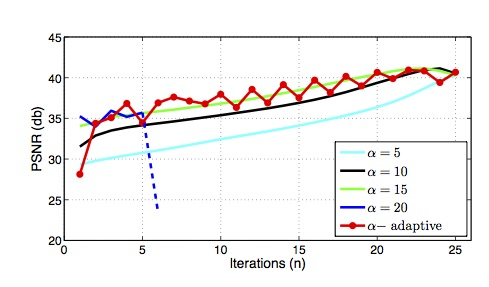
\includegraphics[width = 0.9 \textwidth]{./Diagrams/alpha_accel.jpg}
\caption{Reconstruction performance (expressed in terms of Peak Signal-to-Noise radio) dependence on acceleration coefficients $alpha_n$, for contant value for all iterations $\alpha_n=\alpha$, increasing $\alpha$ brings accelerating convergence, but after some limit, the reconstruction starts to diverge ($\alpha = 20$). Figure taken from \cite{LF-Shearlets} pp. 7}
\label{fig:alpha_accel}
\end{figure}

The approach that we will use and is presented in Algorithm~\ref{alg:lfshearlets1} was proposed by T. Blumensath and M. Davies in 2010 in their article "Normalised Iterative Hard Thresholding; guaranteed stability and performance" \cite{hard-thresholding}. This algorithm applies an iteration-adaptative selection of the parameter given by

$$
\alpha_n=\frac{||\beta_n||_2^2}{||MS^*(\beta_n)||_2^2}
$$

where $\beta_n=S_{\Gamma_n}(y-Mx_n)$ and $S_{\Gamma_n}$ is the shearlet transform decomposition only for coefficients from $\Gamma_n=\textrm{supp}(S(x_n))$; is important to be noticed that $||\cdot||_2$ is the Eucledian norm in the associated $N^2\eta$-dimensional Eucledian space of $\mathbb{R}^{N\times N\times \eta}$ with elements arranged in lexicographic order. The convergence rate of the adaptative selection is also illustrated in Figure~\ref{fig:alpha_accel} and one can see that the adaptation provides high convergence speed and stable reconstruction we refer to the original paper \cite{hard-thresholding} for a more detailed analysis of the convergence and stability conditions, which for our case are fulfilled using the fact that the $0$-Shearlets system form a Parseval Frame. 

\bigskip

As we discurssed in Subsection~\ref{sec:0-Shearlets} we are not obligated to use all the general shearlet transform atoms, instead we favor the use of atoms which are associated with valid directions in EPI; the support of those atomes is illustrated in Figure~\ref{fig:LFshearlets2f}. The scales of the shearlet transform are constructed in dyadic manner, therefore we are choosing $J = \lceil log_2 d_{max}\rceil$ number of scales. In order to perform this programatically using the software Shearlab.jl in every scale we choose $2^{j+1}+1$ shears ($j=0,\ldots, J-1$) to cover the region.

\bigskip

Finally, in the following subsections we will present the resulting inpainted EPIs of the Church data set, as well as the technique that we use to detect lines in the inpainted EPIs and finally compute the depth map. 

\section{Results of sparse EPIs inpaiting}

In order to give the full picture of the EPIs inpainting algorithm implementation and results, we will present the set of ideas that made us take some decisions in the way to design the implementation of the inpainting algorithm.

\bigskip 

As we presented to Section~\ref{sec:Sparse-acquisition} the data set that we used was a series of pictures of a Church, given by the research group of Professor Markus Gross in the Disney Research Center. The data set has 100 different views of the scene, we present in~\ref{fig:first_church},~\ref{fig:second_church} and~\ref{fig:third_church} the 1st, 55th and 100th views of the data set.

\begin{figure}[h!]
\centering
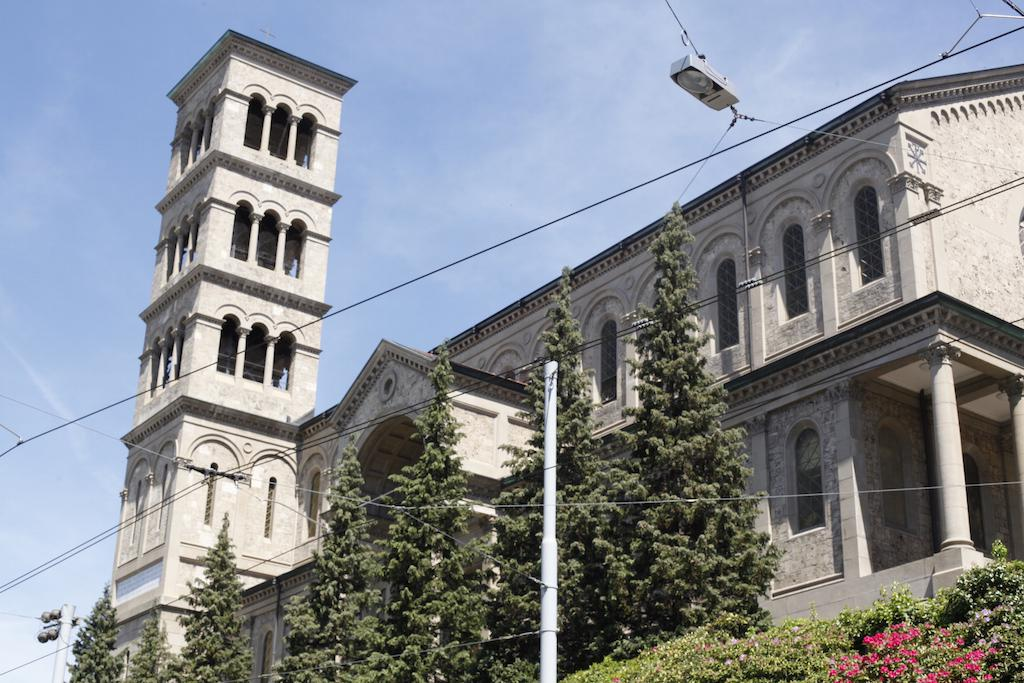
\includegraphics[width = 0.7 \textwidth]{./Diagrams/results/data_set/church_image-raw_0000_lowres.jpg}
\caption{1st picture of the Church Data Set}
\label{fig:first_church}
\end{figure}

\begin{figure}[h!]
\centering
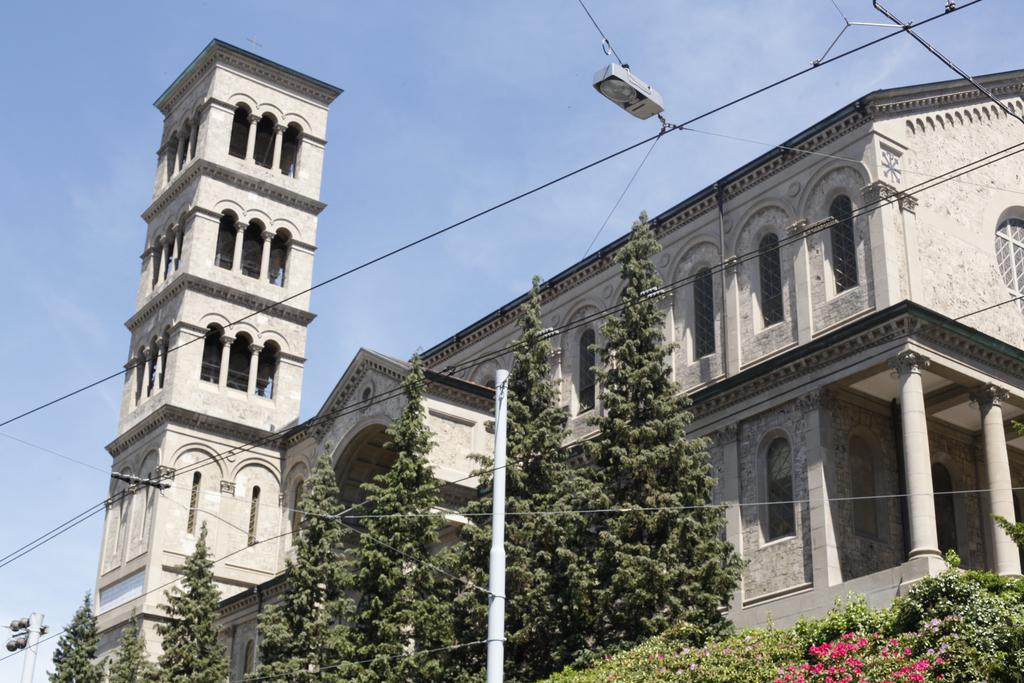
\includegraphics[width = 0.7 \textwidth]{./Diagrams/results/data_set/church_image-raw_0055_lowres.jpg}
\caption{55th picture of the Church Data Set}
\label{fig:second_church}
\end{figure}

\begin{figure}[h!]
\centering
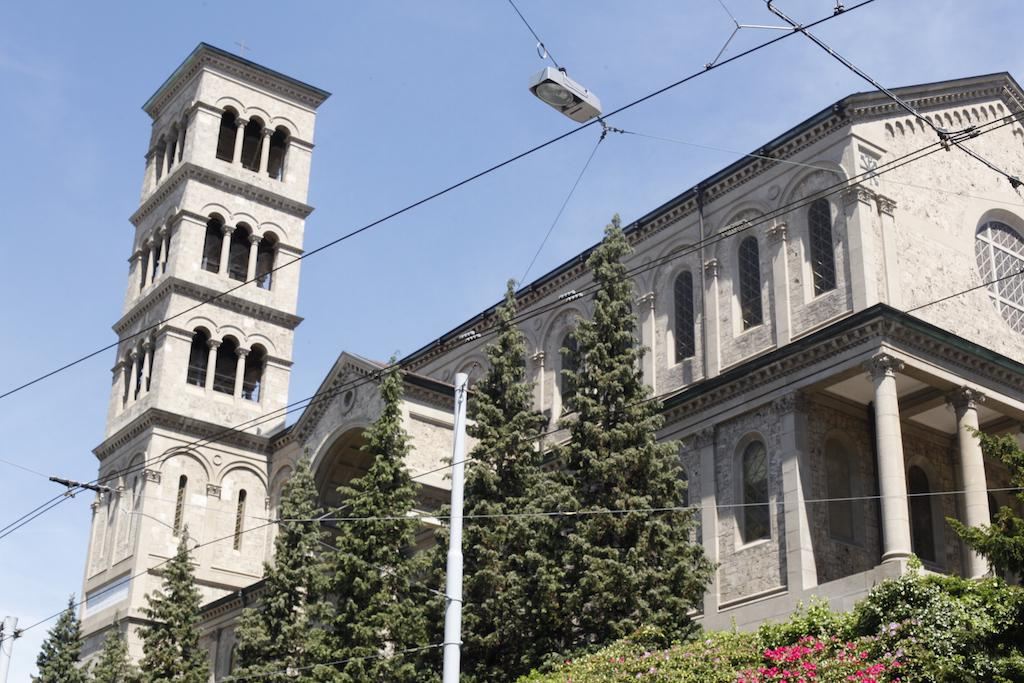
\includegraphics[width = 0.7 \textwidth]{./Diagrams/results/data_set/church_image-raw_0100_lowres.jpg}
\caption{100th picture of the Church Data Set}
\label{fig:third_church}
\end{figure}


\bigskip

\begin{itemize}

\item \textbf{First step (Track Points):} The first step in the implementation was the design the code to track the points; in the Subsection~\ref{sec:proc_track} we presented the followed algorithm (Lucas-Kanade method with Shi-Tomasi corner detector) whose implementation using OpenCV Python's API is presented in Appendix~\ref{sec:Appendix_A} with the results were stored in a data frame that one can find in the repository of this thesis (\url{https://github.com/arsenal9971/MThesis/blob/master/Code_notebooks/church_tracking.csv}) and are presented in Figure~\ref{fig:track_points_church}.

\bigskip

\item \textbf{Second Step (Paint sparse EPIs):}Once we had the data of the tracked points we proceed to paint the EPIs related to fixed $y$-positions in the scenes we used the julia code presented in Appendix~\ref{sec:Appendix_B}, where we used horizontal strips of width $2\epsilon=16.0$ pixels to captures tracked points in the scene at different fixed $y$ positions and follow them along the different views, we also used the same data set to paint the corresponding Sparse Views with a constant disparity between consecutive views $d_{max}=7px$; this maximum disparity was chosen by trying different disparities and pick the best one in terms of the painting speed (the greater the disparity, the less time it takes to paint the sparse EPIs) and the Shearlet-based inpainting performance using a fixed number of iterations (50) in the iterative thresholding algorithm; where we measure the performance mostly in terms of how many lines of the original EPI are captured by our line detection algorithm that will be explained in the next subsection. One can see in Figure~\ref{fig:strip_disparity} the strip of points in the first image that were tracked to perform the benchmark to compute the best disparity parameter for our task; the Figure~\ref{fig:dense_disparity} is the associated densely sampled EPI and the associated sparsely sampled EPIs with different disparities $d_{max}$ are presented in Figure~\ref{fig:first_sparse_disparity},~\ref{fig:second_sparse_disparity},~\ref{fig:third_sparse_disparity} and~\ref{fig:fourth_sparse_disparity}. 

\bigskip

Finally on Figure~\ref{fig:benchmark_line} one can see the different running time obtained for different disparities (clearly the smaller the disparity, the more pictures you need to take and therefore the longest the running time); as we mentioned on Subsection~\ref{sec:proc_track} we used a Macbook Pro with OSX 10.10.5, 8GB of memory, 2.7 GHz Intel Core i5 Processor and Graphic Card Intel Iris Graphics 6100 with 1536 MB of graphic memory (relatively a low end computer system). One can find the whole set of strips, sparse and dense EPIs on \url{https://github.com/arsenal9971/MThesis/tree/master/Diagrams/results/EPIs}, the naming notation that we followed to identify them was \textbf{textfile}=$y_0\_\epsilon\_t_{max}\_d_{max}\_tp\_f.png$ where $y_0$ is the $y$ position of the tracked points on the corresponding strip $\epsilon$ is half the width of the strip, $d_{max}$ is the used disparity for the corresponding sparse EPI, $tp$ is the number of tracked points in the strip and $f$ the number of features corresponding to the tracked points).

\bigskip

\begin{figure}[h!]
\centering
\includegraphics[width = 0.7 \textwidth]{./Diagrams/results/Disparity_benchmark/673_10_102_4_48_8_strip.png}
\caption{Strip of points of width $2\epsilon = 16.0$ px used for the benchmark to choose the disparity $d_{max}$}
\label{fig:strip_disparity}
\end{figure}

\begin{figure}[h!]
\centering
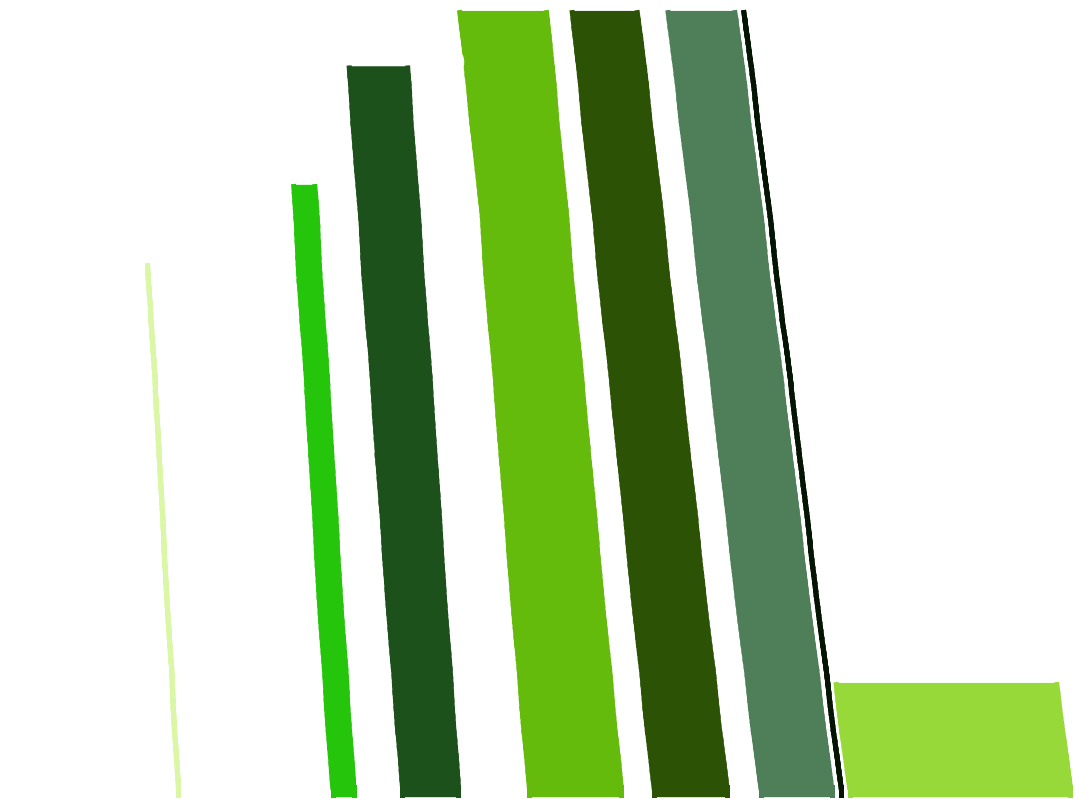
\includegraphics[width = 0.7 \textwidth]{./Diagrams/results/Disparity_benchmark/673_10_102_4_48_8_dense.png}
\caption{Densely sampled EPI associated to the points in the strip on Figure~\ref{fig:strip_disparity}}
\label{fig:dense_disparity}
\end{figure}

\begin{figure}[h!]
\centering
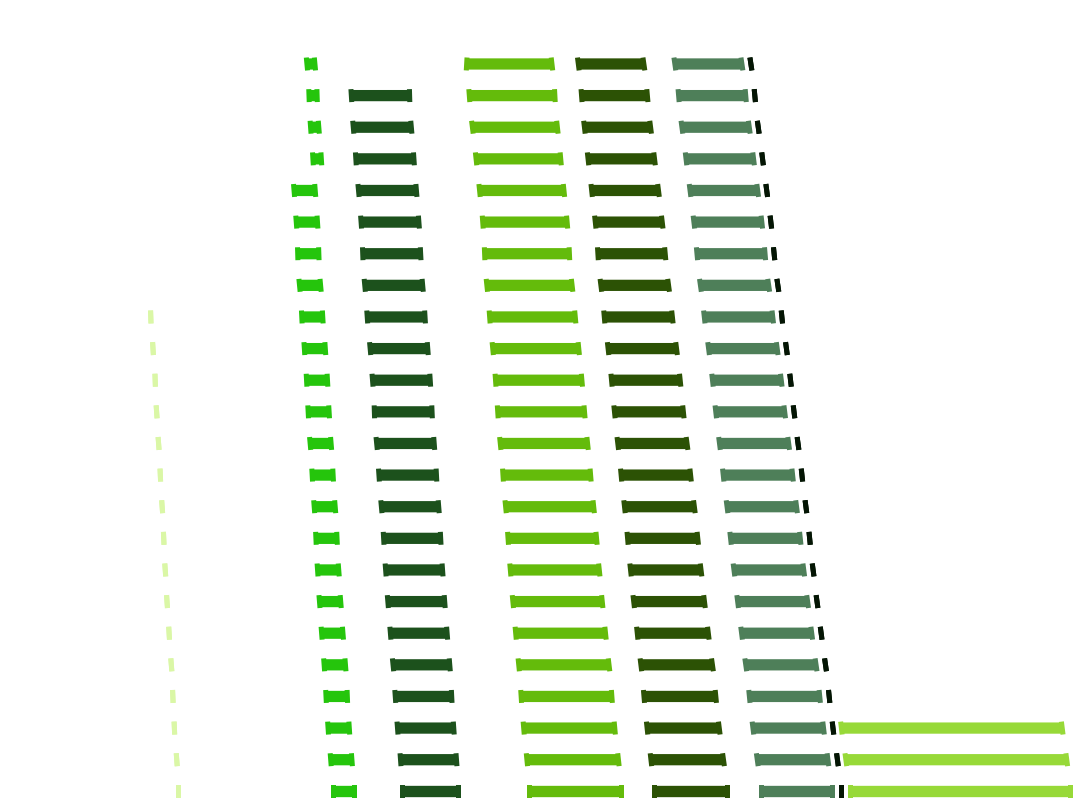
\includegraphics[width = 0.7 \textwidth]{./Diagrams/results/Disparity_benchmark/673_10_102_4_48_8_sparse.png}
\caption{Sparsely sampled EPI associated to the disparity $d_{max} = 4$ px}
\label{fig:first_sparse_disparity}
\end{figure}

\begin{figure}[h!]
\centering
\includegraphics[width = 0.7 \textwidth]{./Diagrams/results/Disparity_benchmark/673_10_102_7_48_8_sparse.png}
\caption{Sparsely sampled EPI associated to the disparity $d_{max} = 7$ px}
\label{fig:second_sparse_disparity}
\end{figure}

\begin{figure}[h!]
\centering
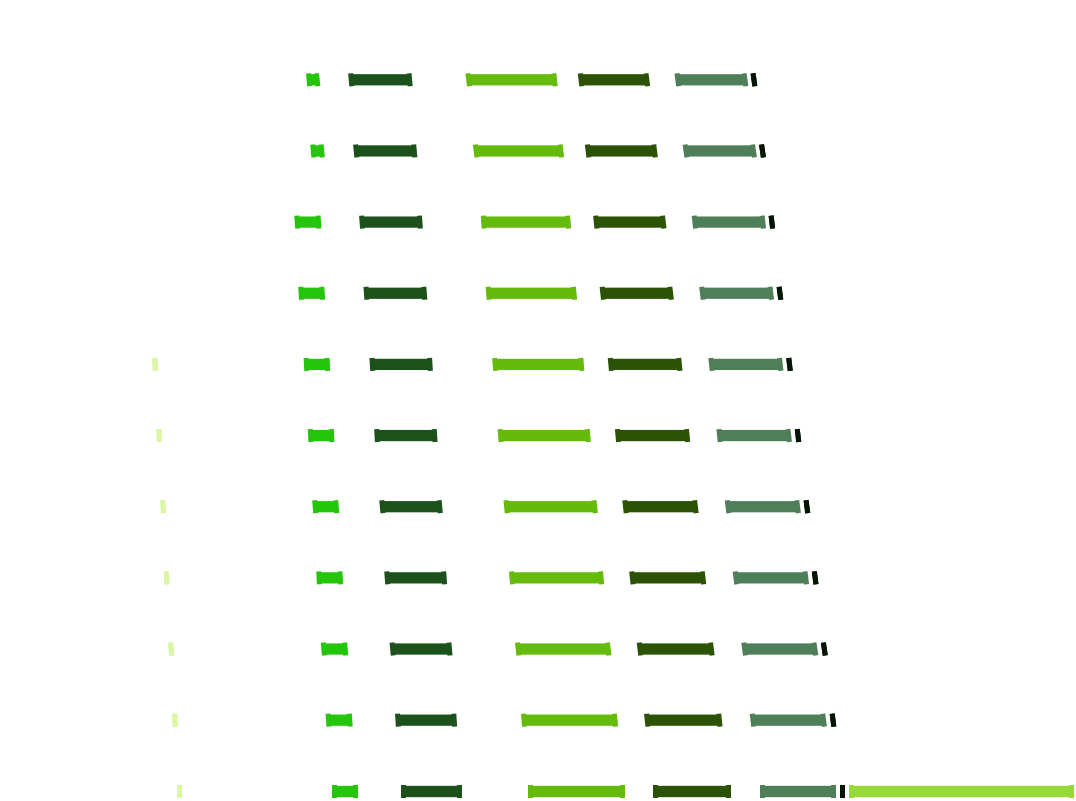
\includegraphics[width = 0.7 \textwidth]{./Diagrams/results/Disparity_benchmark/673_10_102_9_48_8_sparse.png}
\caption{Sparsely sampled EPI associated to the disparity $d_{max}=9$ px}
\label{fig:third_sparse_disparity}
\end{figure}

\begin{figure}[h!]
\centering
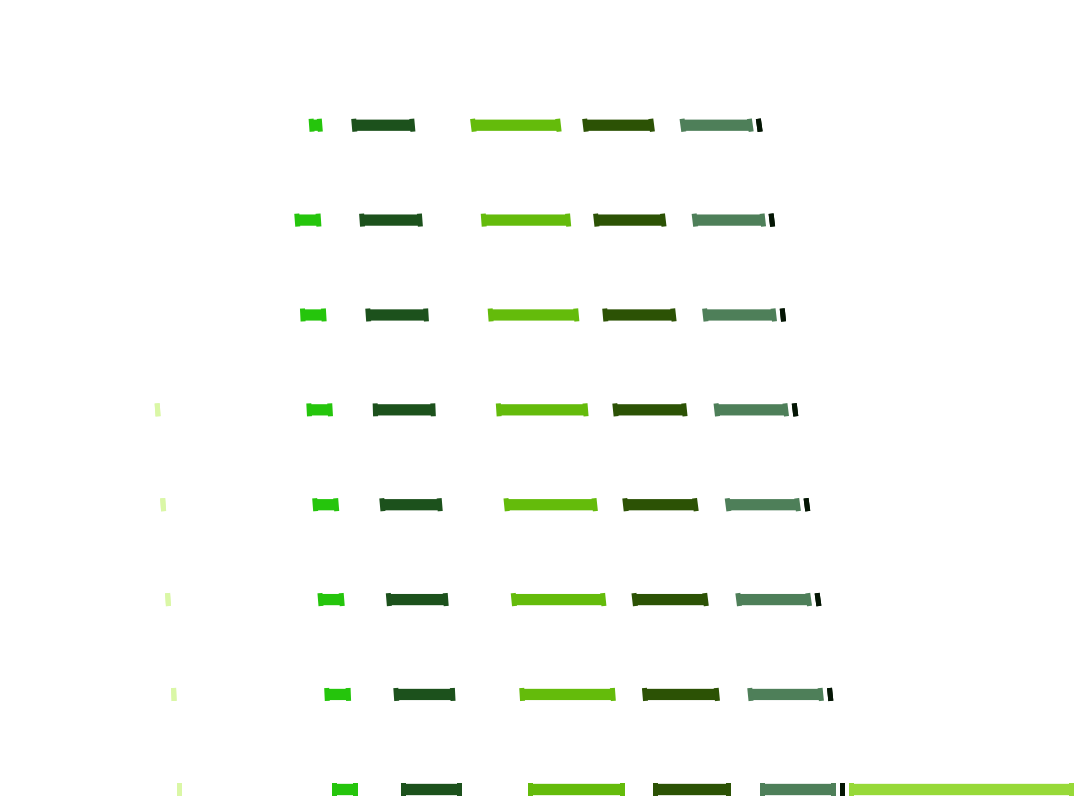
\includegraphics[width = 0.7 \textwidth]{./Diagrams/results/Disparity_benchmark/673_10_102_12_48_8_sparse.png}
\caption{Sparsely sampled EPI associated to the disparity $d_{max}=12$ px}
\label{fig:fourth_sparse_disparity}
\end{figure}

\begin{figure}[h!]
\centering
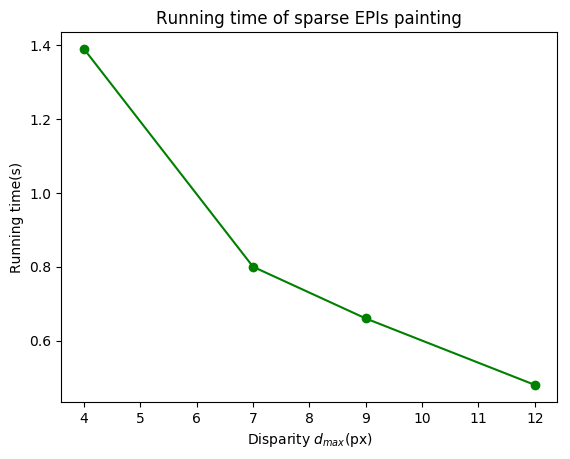
\includegraphics[width = 0.7 \textwidth]{./Diagrams/results/Disparity_benchmark/sparse_painting_benchmark.png}
\caption{Running time of painting of sparsely sampled EPIs with different disparities}
\label{fig:benchmark_line}
\end{figure}


\bigskip

One can also see in Figures~\ref{fig:first_lines_disparity},~\ref{fig:second_lines_disparity},~\ref{fig:third_lines_disparity} and~\ref{fig:fourth_lines_disparity} the lines detected in different inpainted EPIs corresponding to the same dense EPI, with different views disparity $d_max$, one can see that the important features are detected when $d_{max}=4$ and $d_{max}=7$ while when $d_{max}$ is bigger some lines are lost. 

\begin{figure}[h!]
\centering
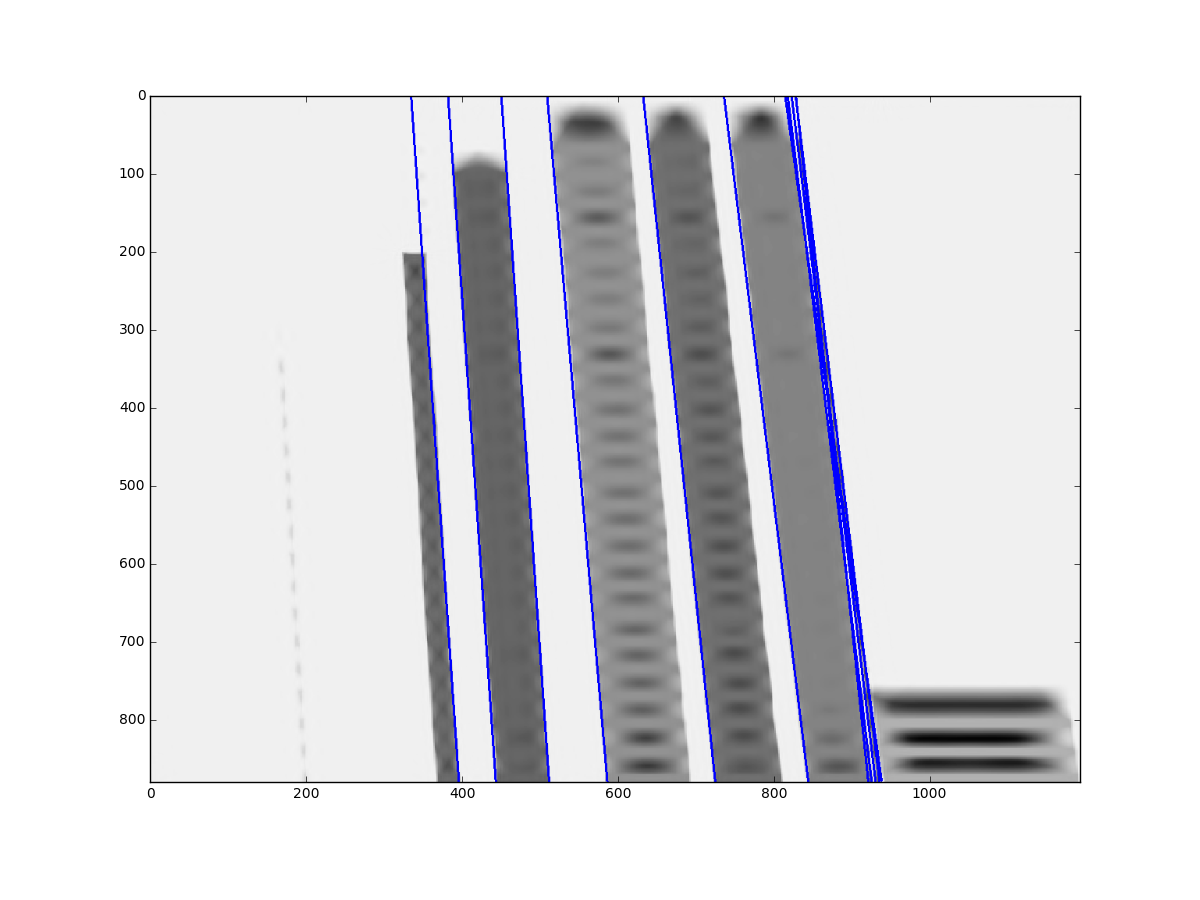
\includegraphics[width = 0.7 \textwidth]{./Diagrams/results/Disparity_benchmark/673_10_102_4_48_8_lines.png}
\caption{Lines detected in an inpainted using disparity $d_{max} = 4$ px}
\label{fig:first_lines_disparity}
\end{figure}

\begin{figure}[h!]
\centering
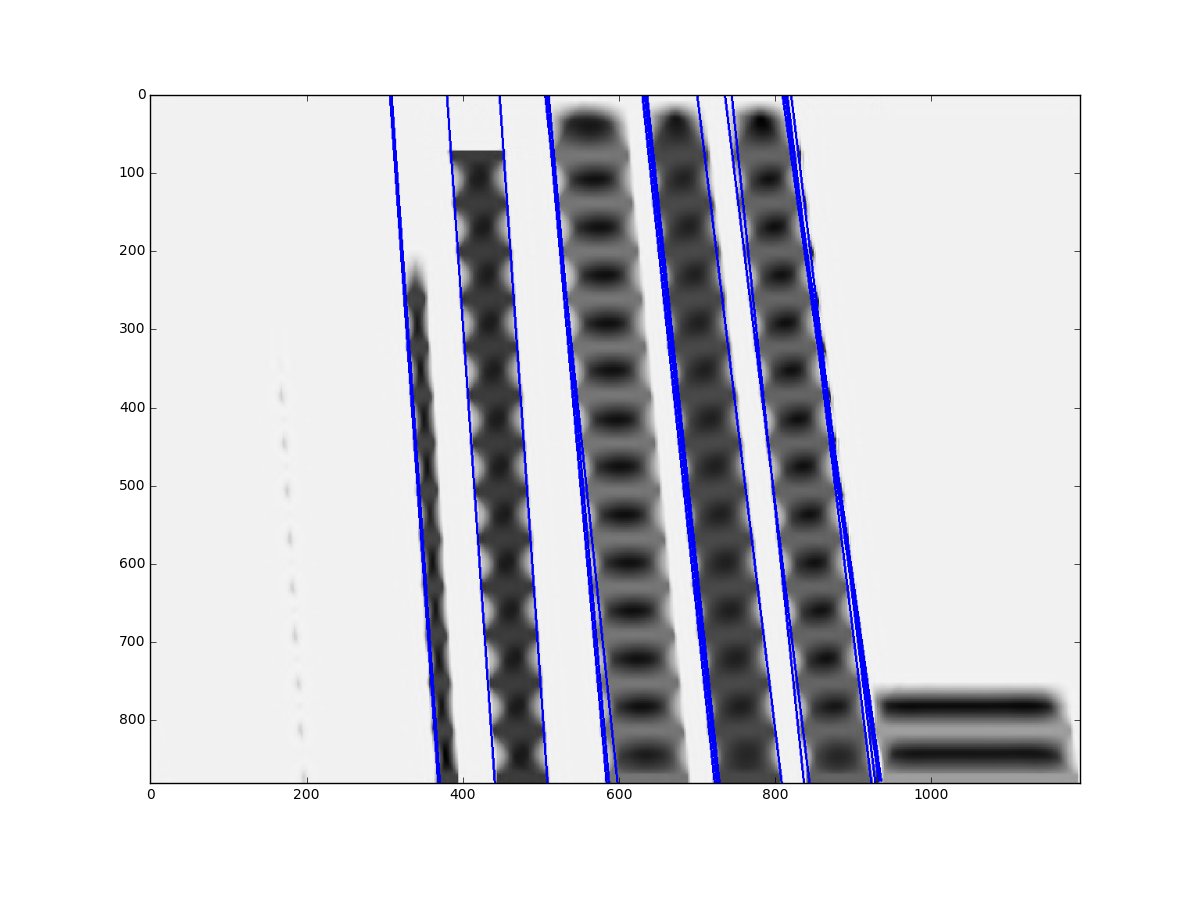
\includegraphics[width = 0.7 \textwidth]{./Diagrams/results/Disparity_benchmark/673_10_102_7_48_8_lines.png}
\caption{Lines detected in an inpainted using disparity $d_{max} = 7$ px}
\label{fig:second_lines_disparity}
\end{figure}

\begin{figure}[h!]
\centering
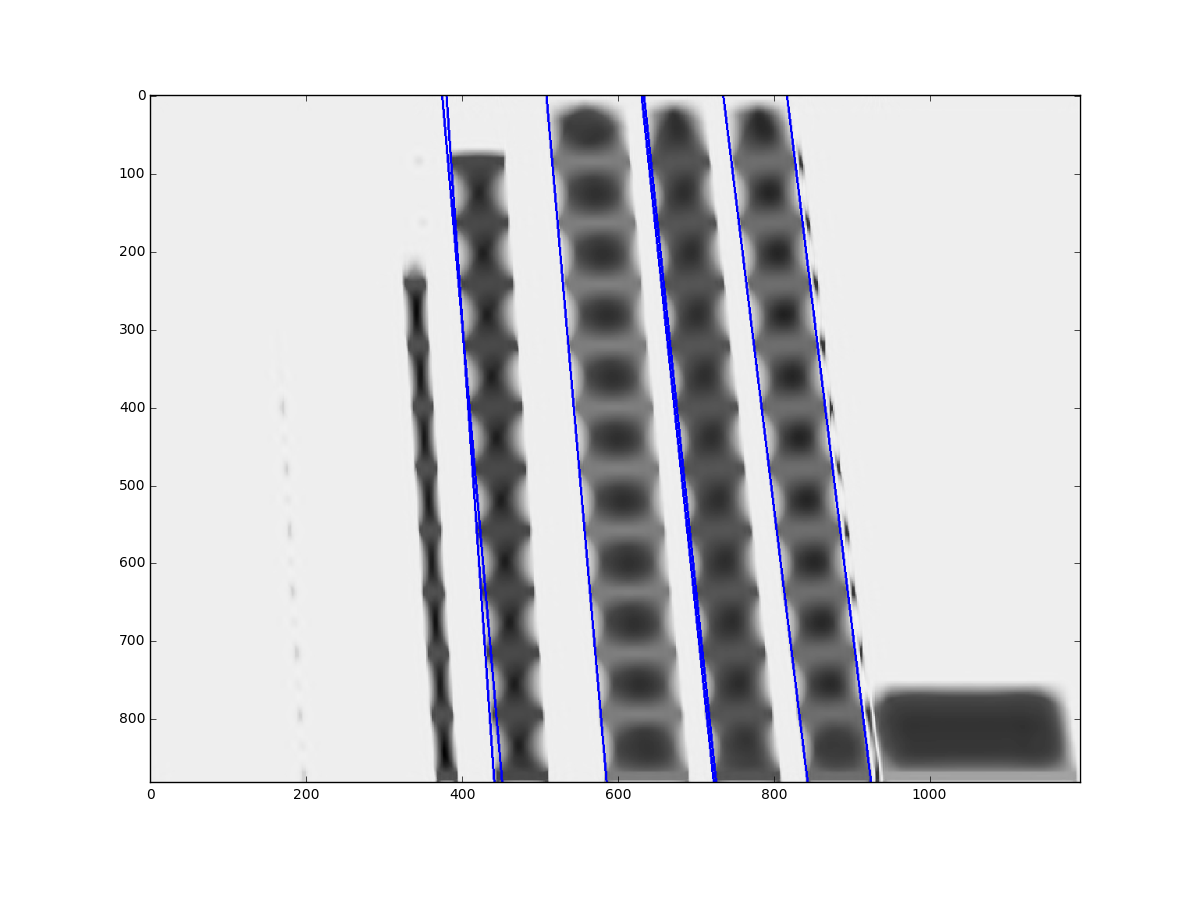
\includegraphics[width = 0.7 \textwidth]{./Diagrams/results/Disparity_benchmark/673_10_102_9_48_8_lines.png}
\caption{Lines detected in an inpainted using disparity $d_{max} = 9$ px}
\label{fig:third_lines_disparity}
\end{figure}

\begin{figure}[h!]
\centering
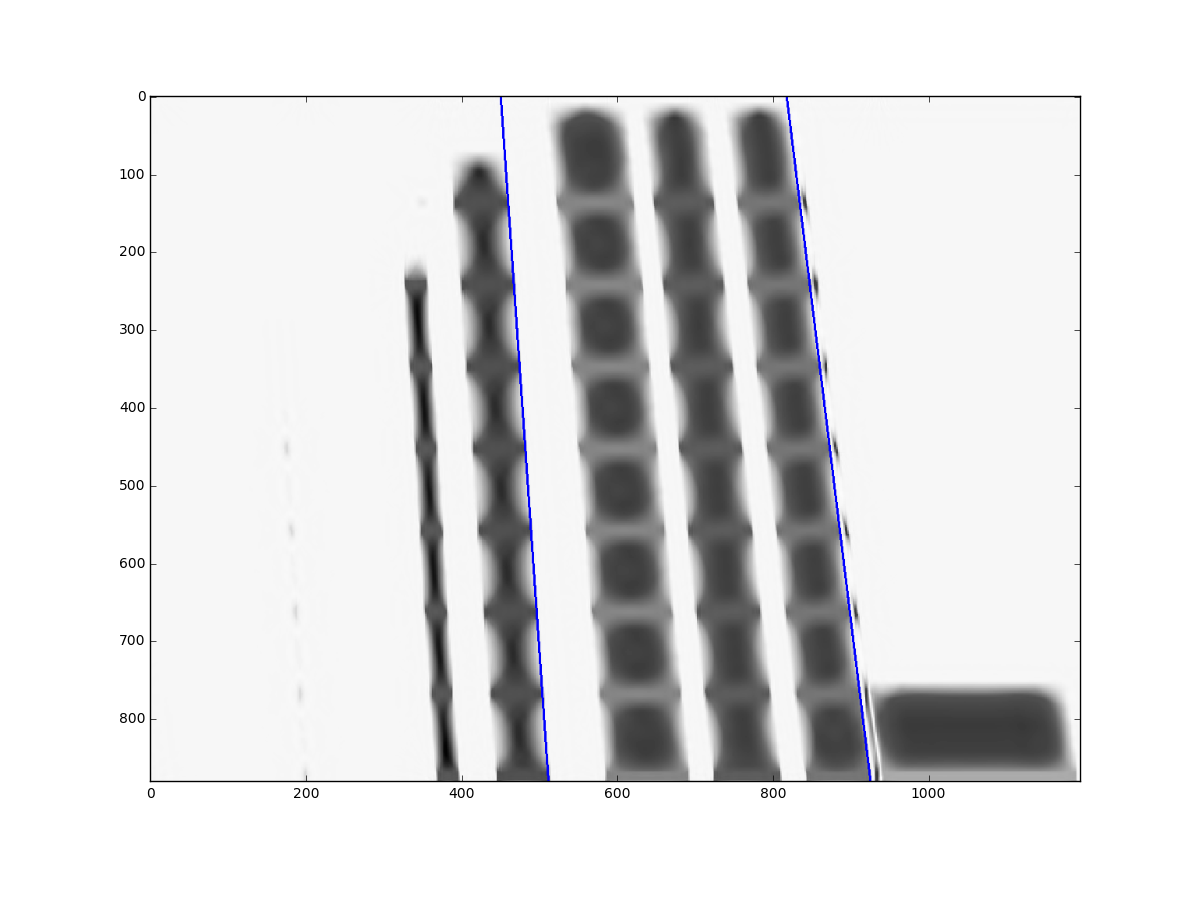
\includegraphics[width = 0.7 \textwidth]{./Diagrams/results/Disparity_benchmark/673_10_102_12_48_8_lines.png}
\caption{Lines detected in an inpainted using disparity $d_{max} = 12$ px}
\label{fig:fourth_lines_disparity}
\end{figure}

\begin{figure}[h!]
\centering
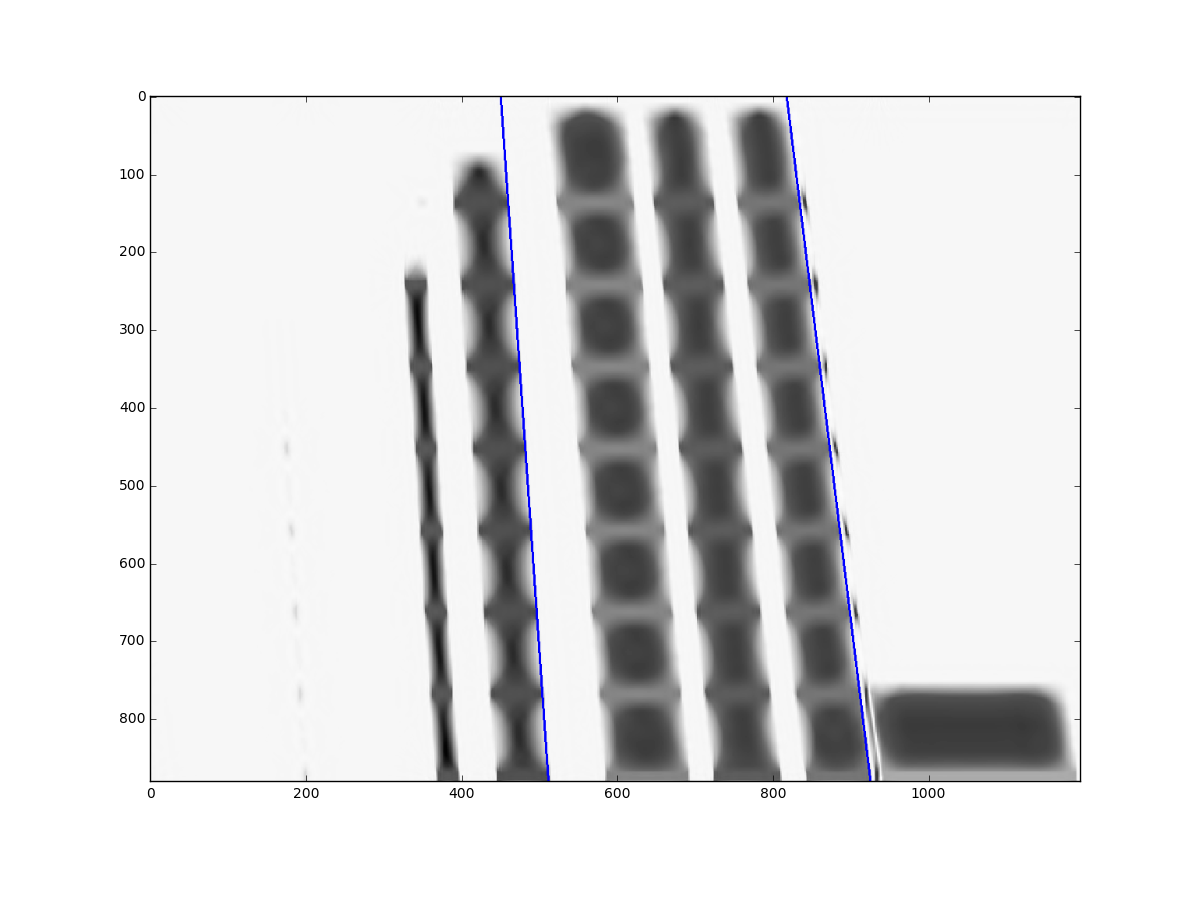
\includegraphics[width = 0.7 \textwidth]{./Diagrams/results/Disparity_benchmark/673_10_102_12_48_8_lines.png}
\caption{Lines detected in an inpainted using disparity $d_{max} = 12$ px}
\label{fig:fourth_lines_disparity}
\end{figure}

\begin{figure}[h!]
\centering
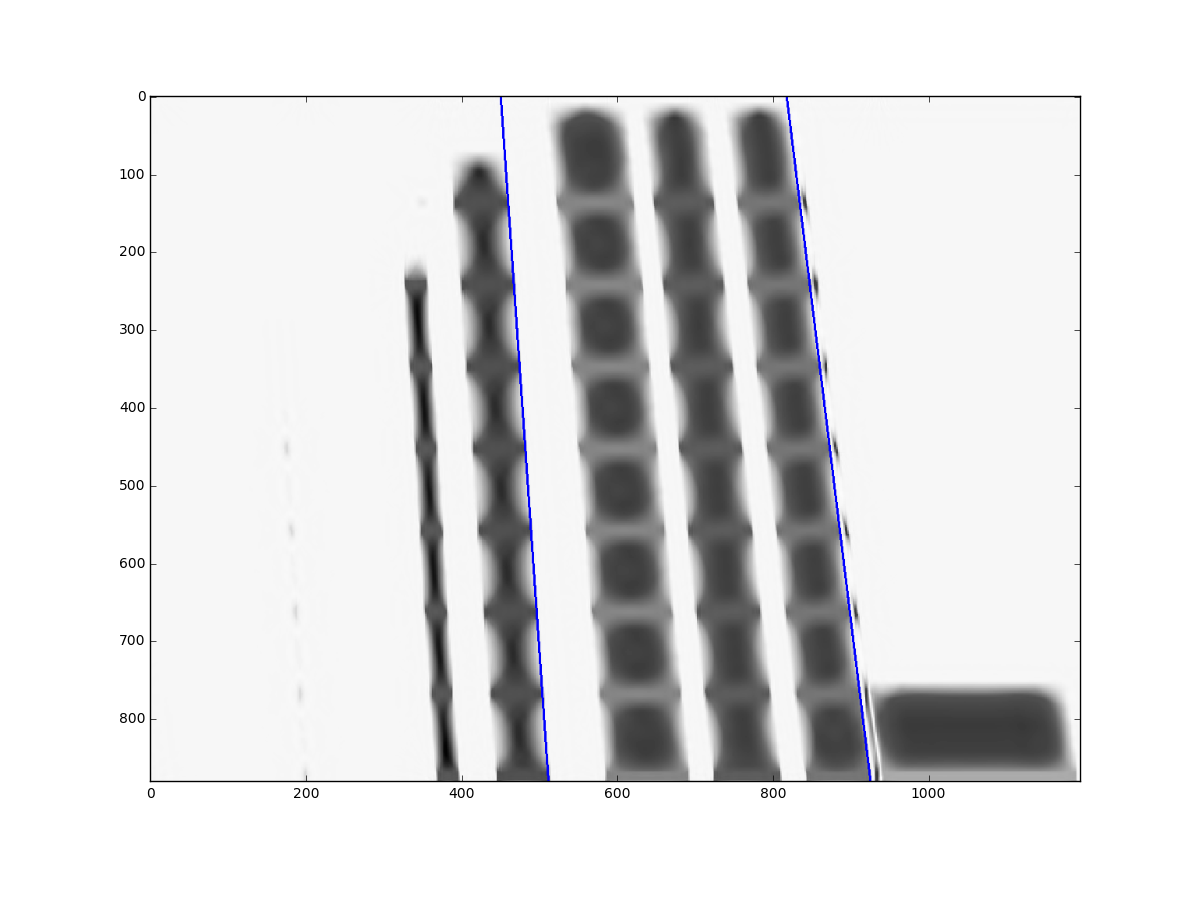
\includegraphics[width = 0.7 \textwidth]{./Diagrams/results/Disparity_benchmark/673_10_102_12_48_8_lines.png}
\caption{Lines detected in an inpainted using disparity $d_{max} = 12$ px}
\label{fig:fourth_lines_disparity}
\end{figure}

\item \textbf{Third step (Inpaint sparse EPIs):} After paint all the sparsely sampled EPIs corresponding to different horizontal strips of width $16.0$px whose union cover all the tracked points, we inpainted to recover a densely sampled EPIs and therefore we can finally compute the depth map by computing the slopes of the different lines in the EPIs. As we already mentioned on the last section, in order to perform the minimization problem associated with the inpainting algorithm we used iterative hard thresholding with a $0$-Shearlet system as sparsifying system whose code we can find on Appendix~\ref{sec:Appendix_C} and was implemented using julia programming language with the libraries PyPlot.jl and Shearlab.jl. 

\bigskip

We choose some of the best EPIs (corresponding to strips that capture an important number of tracked points) to show here (see Figures~\ref{fig:strip1} to~\ref{fig:inpainted5}), but to compute the depth map we used all the inpainted EPIs that can be found on \url{https://github.com/arsenal9971/MThesis/tree/master/Diagrams/results/Inpainted} that follow the same naming notation as the dense EPIs, sparse EPIs and strips).

\bigskip

We are not looking here for high resolution light fields but for fast recoverable light fields so we imported in julia the sparse EPIs with a horizontal size of $n=512$ pixels, using the same computer system as already mentioned the inpainting of the EPIs with 50 iterations took 19.15 seconds when using a fixed acceleration parameter $\alpha = 1$, whereas it took 15.5 seconds when using a the adaptive acceleration parameter defined on Algorithm~\ref{alg:lfshearlets1}.

\begin{figure}[h!]
\centering
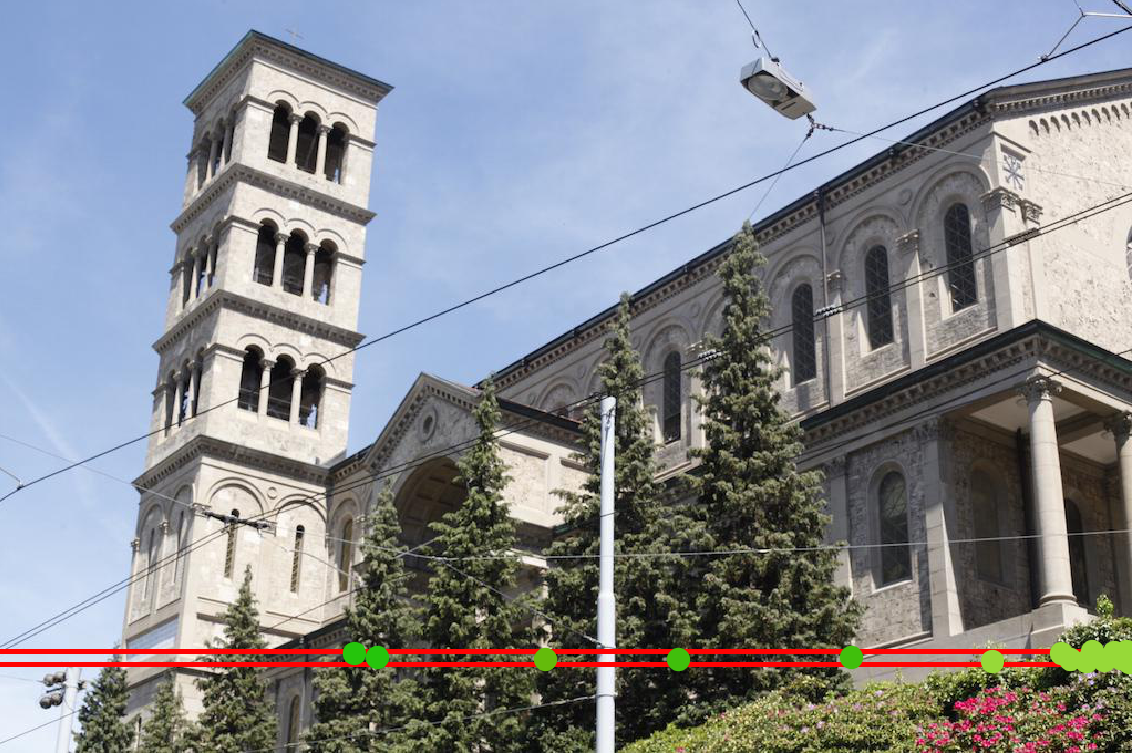
\includegraphics[width = 0.7 \textwidth]{./Diagrams/results/EPIs/392_8_102_7_15_4_strip.png}
\caption{Strip with tracked points}
\label{fig:strip1}
\end{figure}

\begin{figure}[h!]
\centering

\includegraphics[width = 0.7 \textwidth]{./Diagrams/results/EPIs/392_8_102_7_15_4_dense.png}
\caption{Dense EPI corresponding to the strip on Figure~\ref{fig:strip1}}
\label{fig:dense1}
\end{figure}

\begin{figure}[h!]
\centering
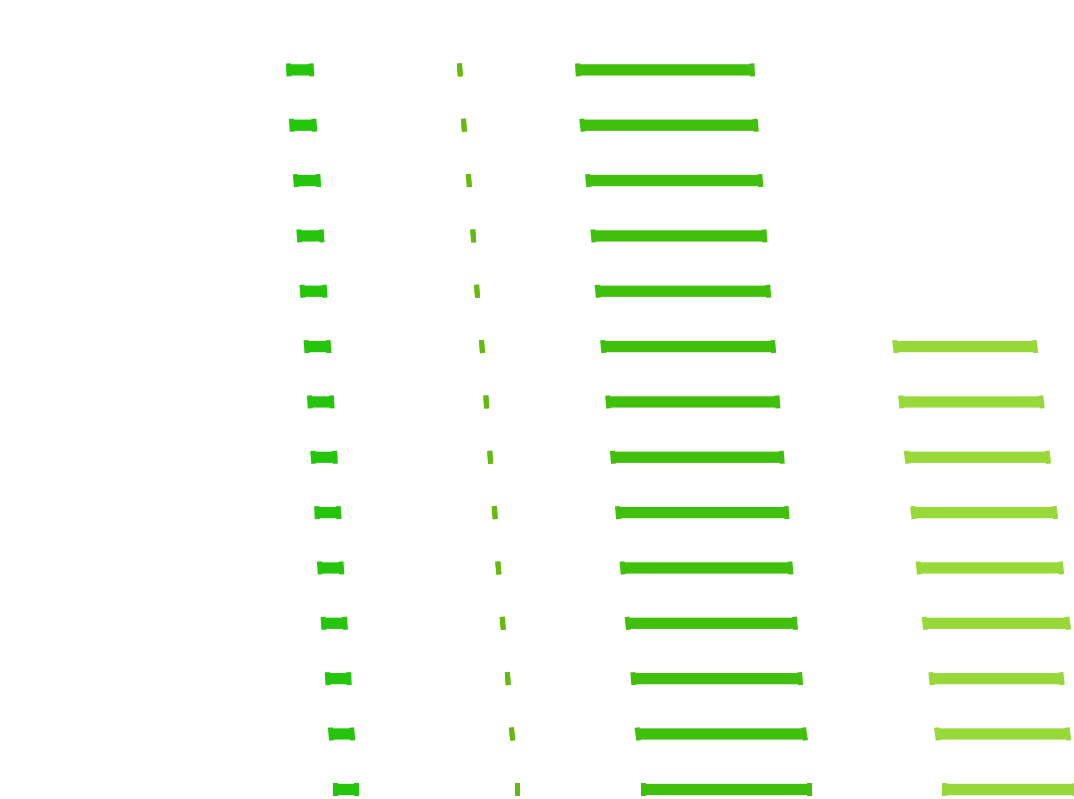
\includegraphics[width = 0.7 \textwidth]{./Diagrams/results/EPIs/392_8_102_7_15_4_sparse.png}
\caption{Sparse EPI corresponding to the strip on Figure~\ref{fig:strip1}}
\label{fig:sparse1}
\end{figure}

\begin{figure}[h!]
\centering
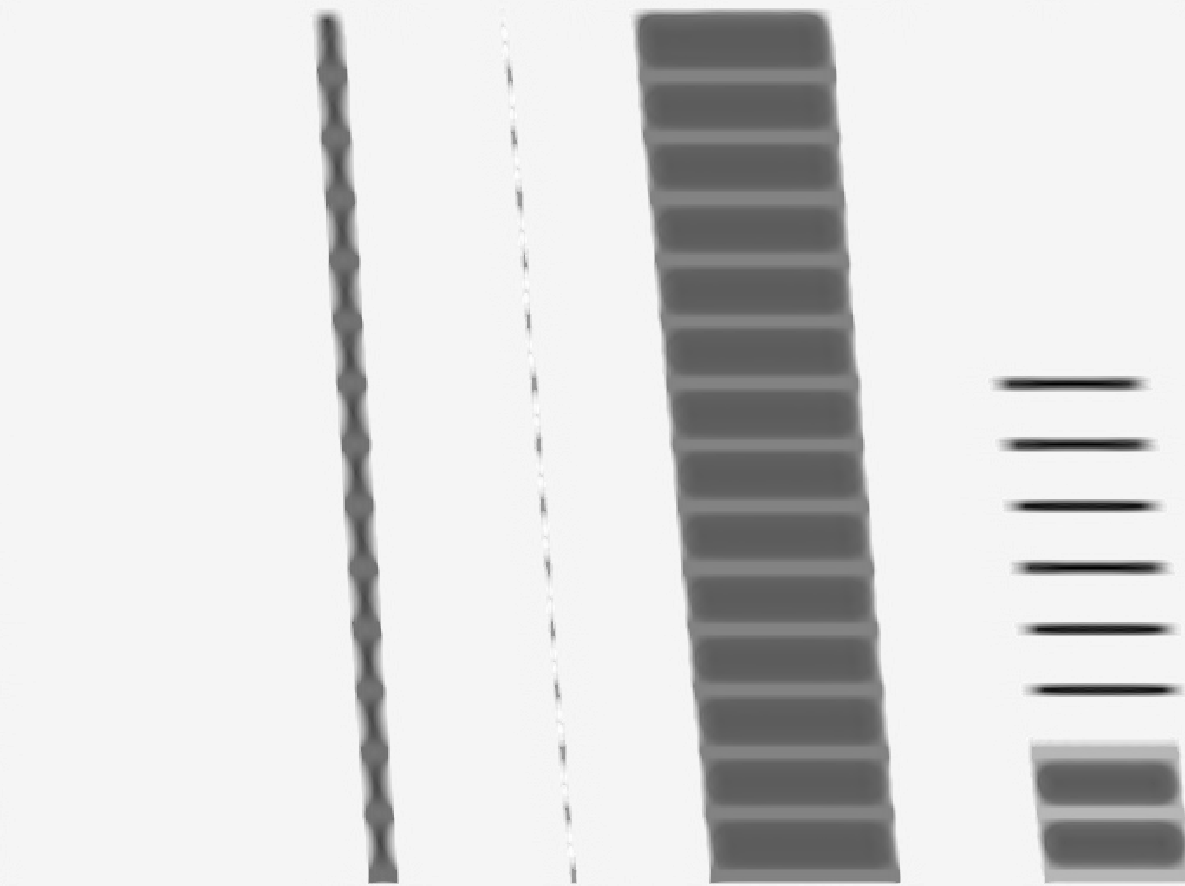
\includegraphics[width = 0.7 \textwidth]{./Diagrams/results/Inpainted/392_8_102_7_15_4_inpainted.png}
\caption{Inpainted EPI corresponding to the strip on Figure~\ref{fig:strip1}}
\label{fig:inpainted1}
\end{figure}


\begin{figure}[h!]
\centering
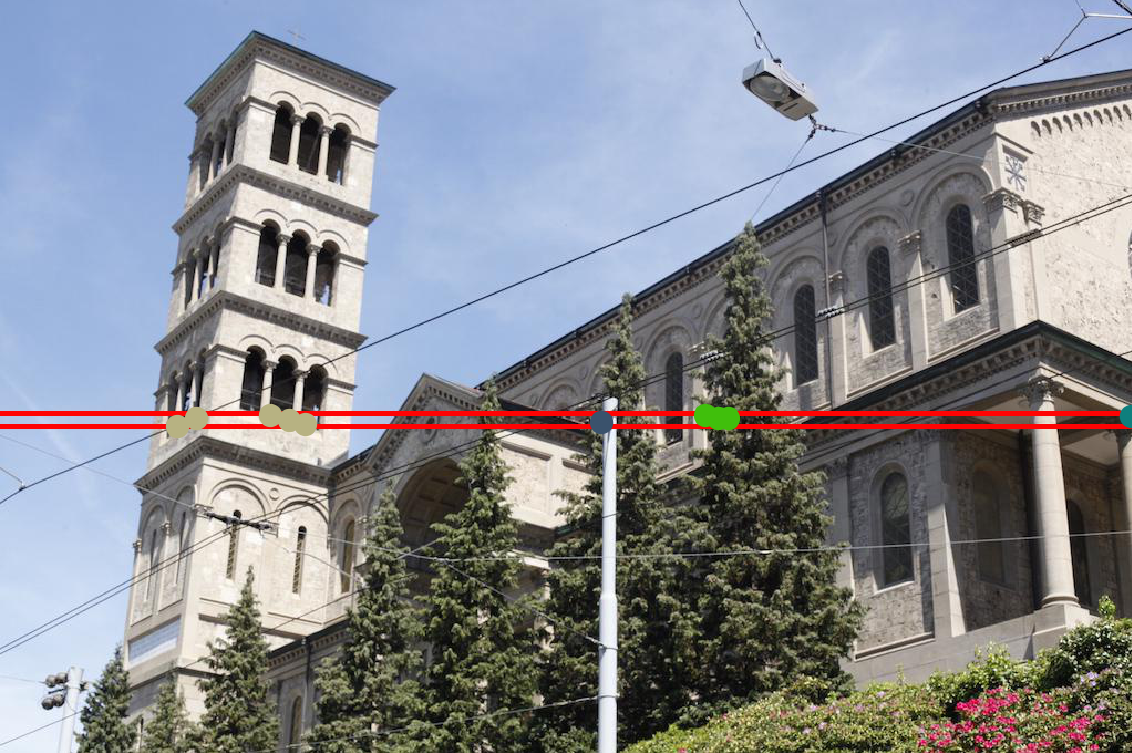
\includegraphics[width = 0.7 \textwidth]{./Diagrams/results/EPIs/424_8_102_7_10_4_strip.png}
\caption{Strip with tracked points}
\label{fig:strip2}
\end{figure}

\begin{figure}[h!]
\centering
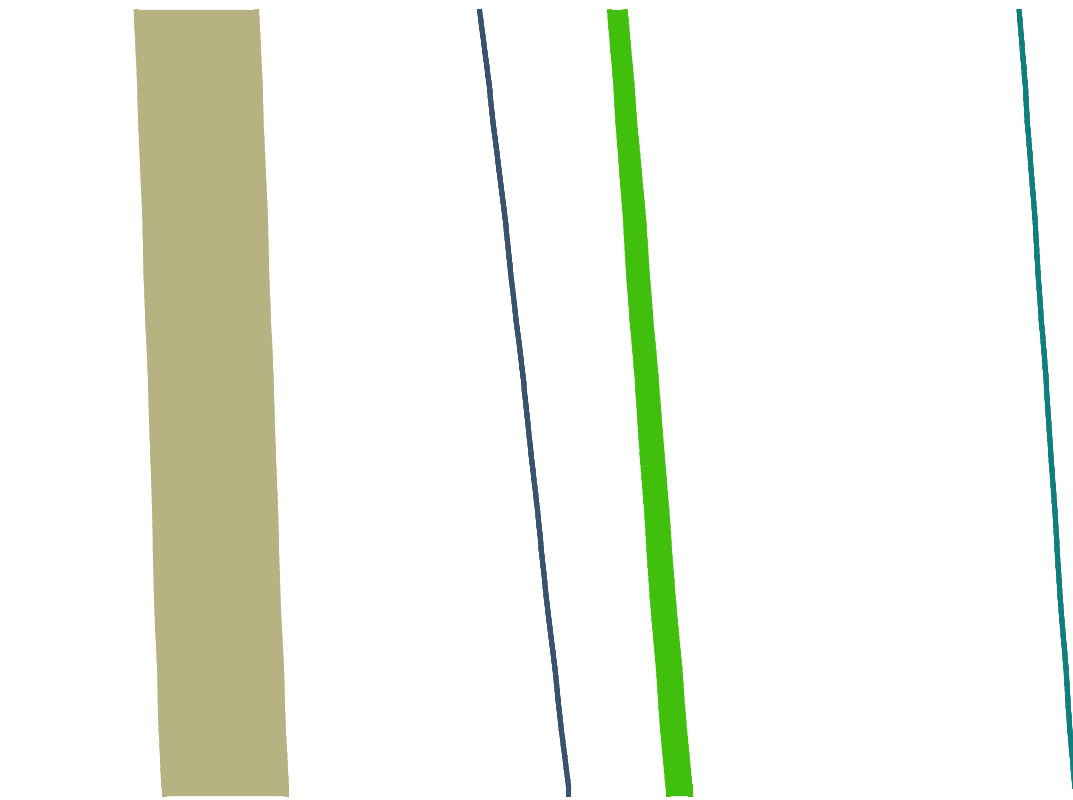
\includegraphics[width = 0.7 \textwidth]{./Diagrams/results/EPIs/424_8_102_7_10_4_dense.png}
\caption{Dense EPI corresponding to the strip on Figure~\ref{fig:strip2}}
\label{fig:dense2}
\end{figure}

\begin{figure}[h!]
\centering
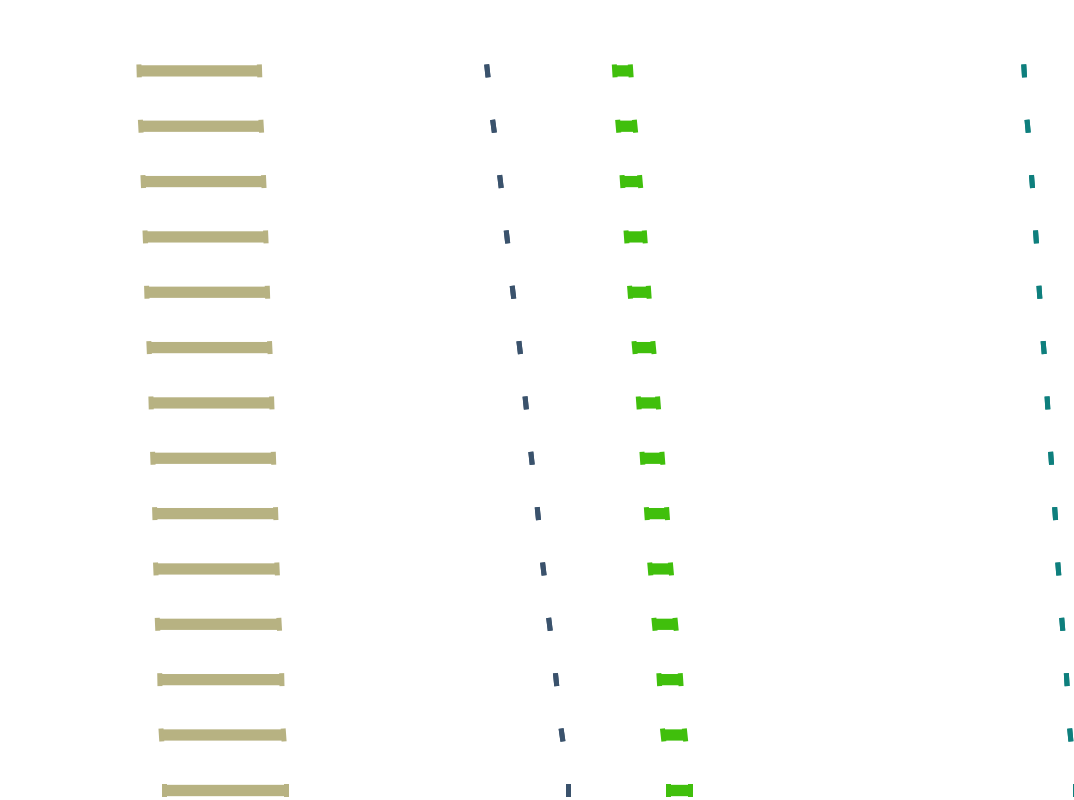
\includegraphics[width = 0.7 \textwidth]{./Diagrams/results/EPIs/424_8_102_7_10_4_sparse.png}
\caption{Sparse EPI corresponding to the strip on Figure~\ref{fig:strip2}}
\label{fig:sparse2}
\end{figure}

\begin{figure}[h!]
\centering
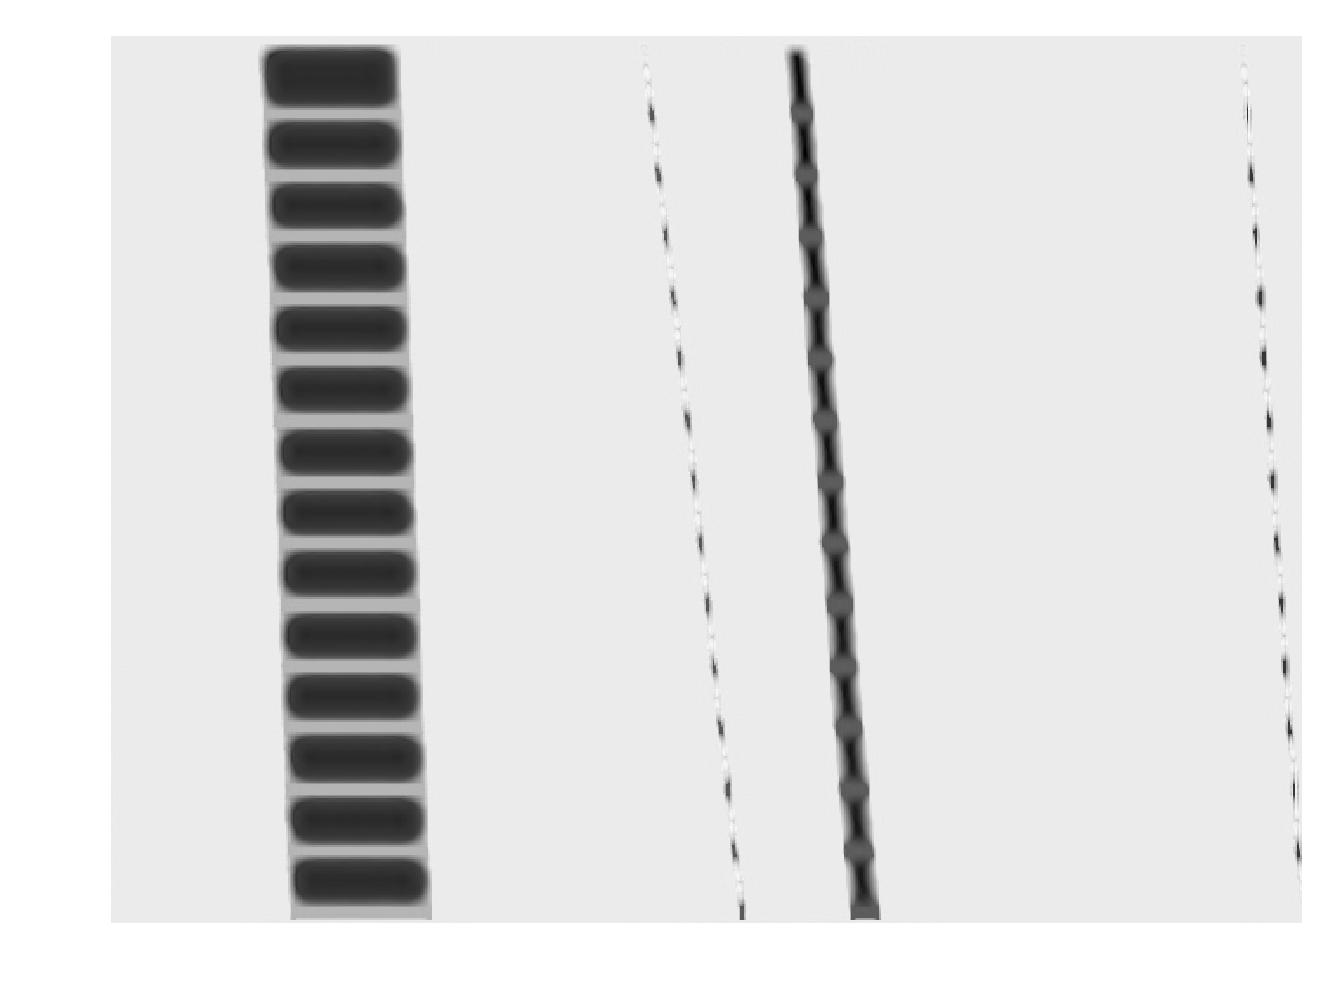
\includegraphics[width = 0.7 \textwidth]{./Diagrams/results/Inpainted/424_8_102_7_10_4_inpainted.png}
\caption{Inpainted EPI corresponding to the strip on Figure~\ref{fig:strip2}}
\label{fig:inpainted2}
\end{figure}

\begin{figure}[h!]
\centering
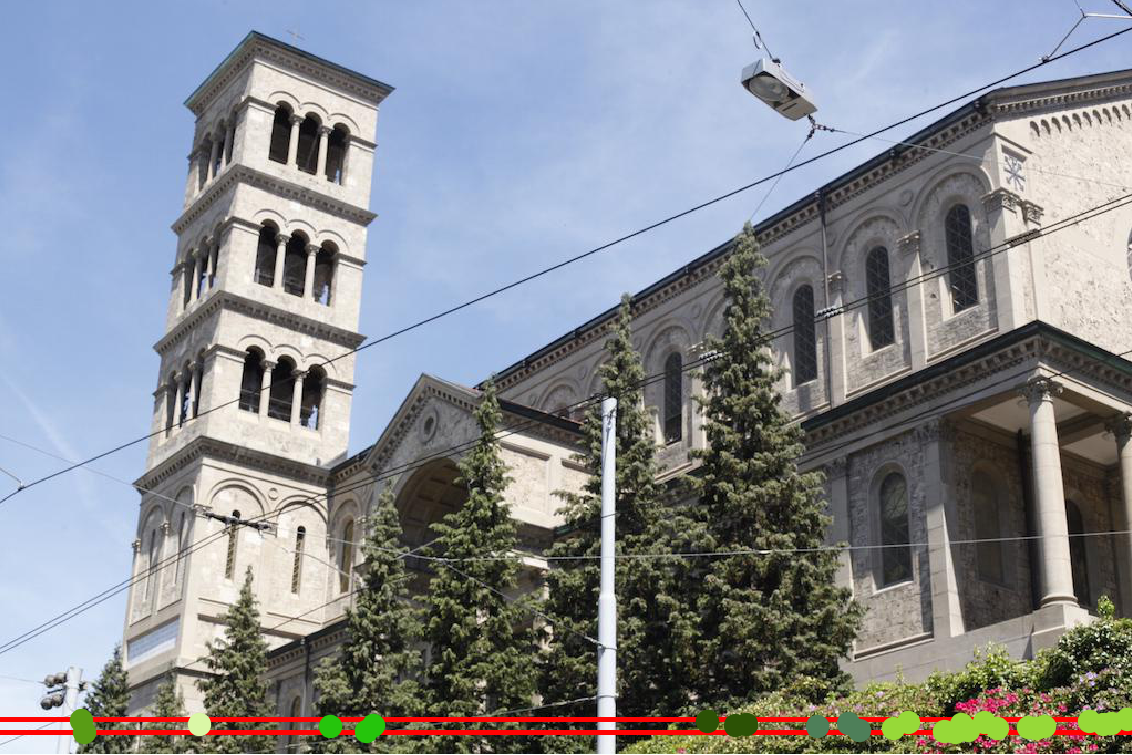
\includegraphics[width = 0.7 \textwidth]{./Diagrams/results/EPIs/306_8_102_7_27_6_strip.png}
\caption{Strip with tracked points}
\label{fig:strip3}
\end{figure}

\begin{figure}[h!]
\centering
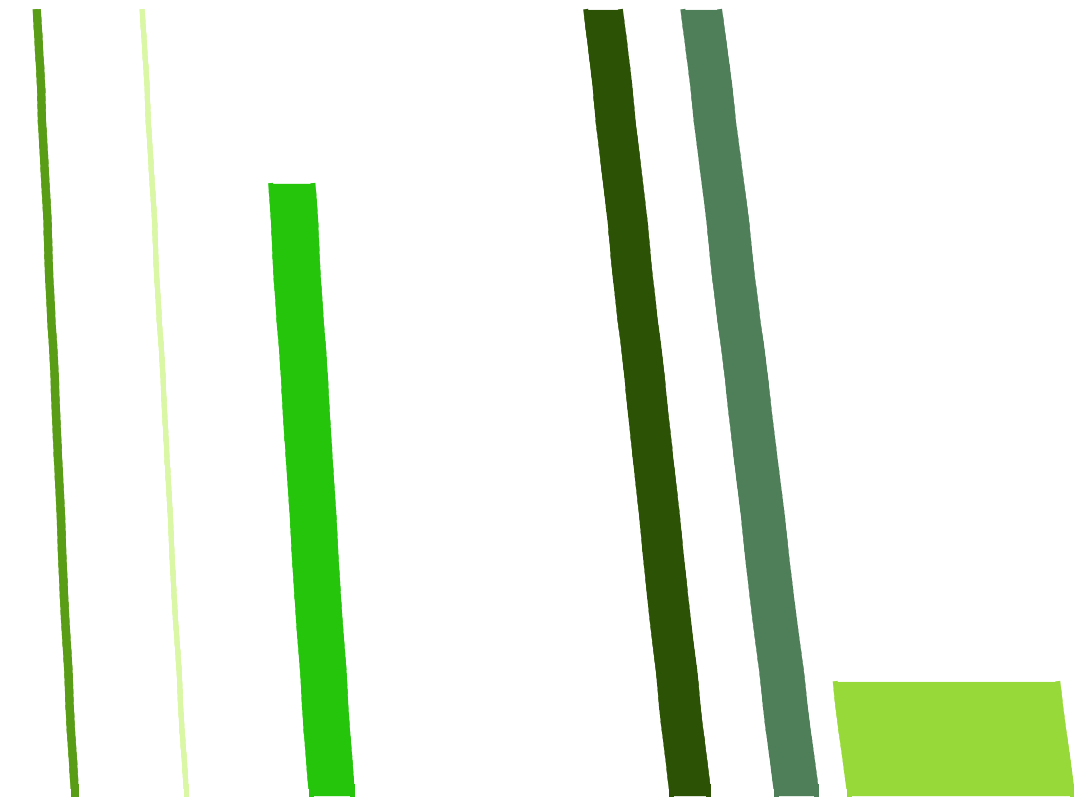
\includegraphics[width = 0.7 \textwidth]{./Diagrams/results/EPIs/306_8_102_7_27_6_dense.png}
\caption{Dense EPI corresponding to the strip on Figure~\ref{fig:strip3}}
\label{fig:dense3}
\end{figure}

\begin{figure}[h!]
\centering
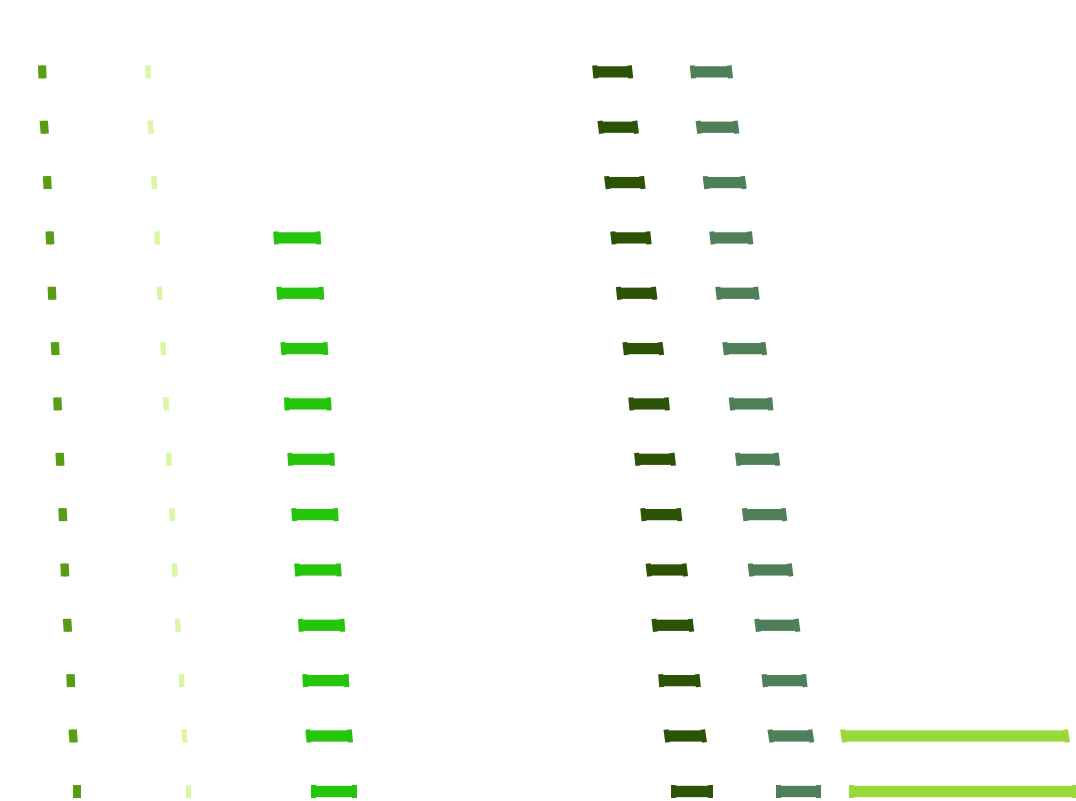
\includegraphics[width = 0.7 \textwidth]{./Diagrams/results/EPIs/306_8_102_7_27_6_sparse.png}
\caption{Sparse EPI corresponding to the strip on Figure~\ref{fig:strip3}}
\label{fig:sparse3}
\end{figure}

\begin{figure}[h!]
\centering
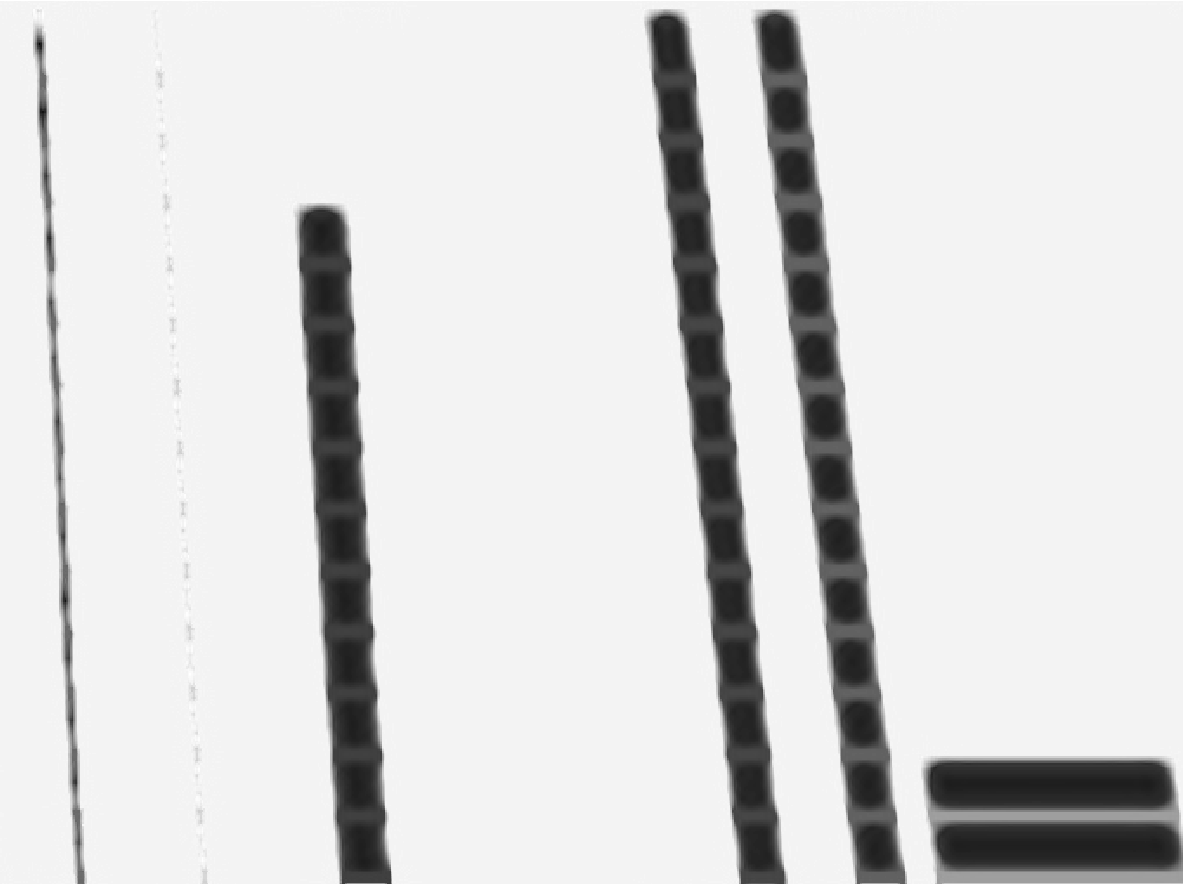
\includegraphics[width = 0.7 \textwidth]{./Diagrams/results/Inpainted/306_8_102_7_27_6_inpainted.png}
\caption{Inpainted EPI corresponding to the strip on Figure~\ref{fig:strip3}}
\label{fig:inpainted3}
\end{figure}

\begin{figure}[h!]
\centering
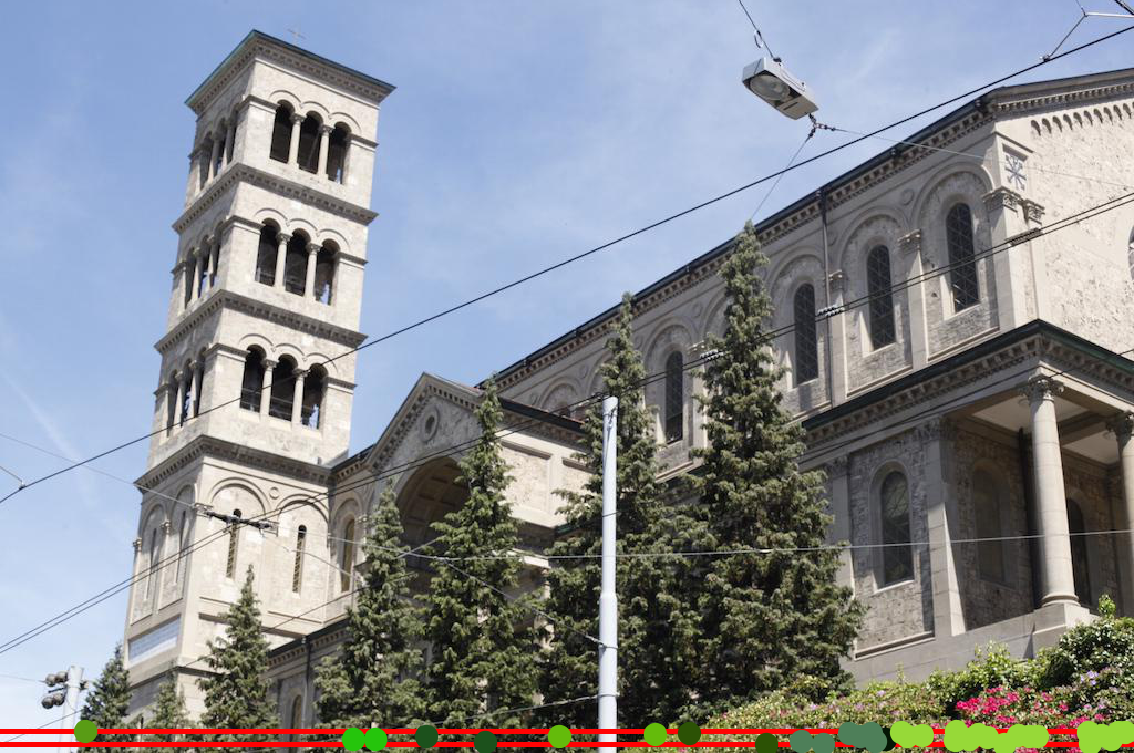
\includegraphics[width = 0.7 \textwidth]{./Diagrams/results/EPIs/292_8_102_7_34_8_strip.png}
\caption{Strip with tracked points}
\label{fig:strip4}
\end{figure}

\begin{figure}[h!]
\centering
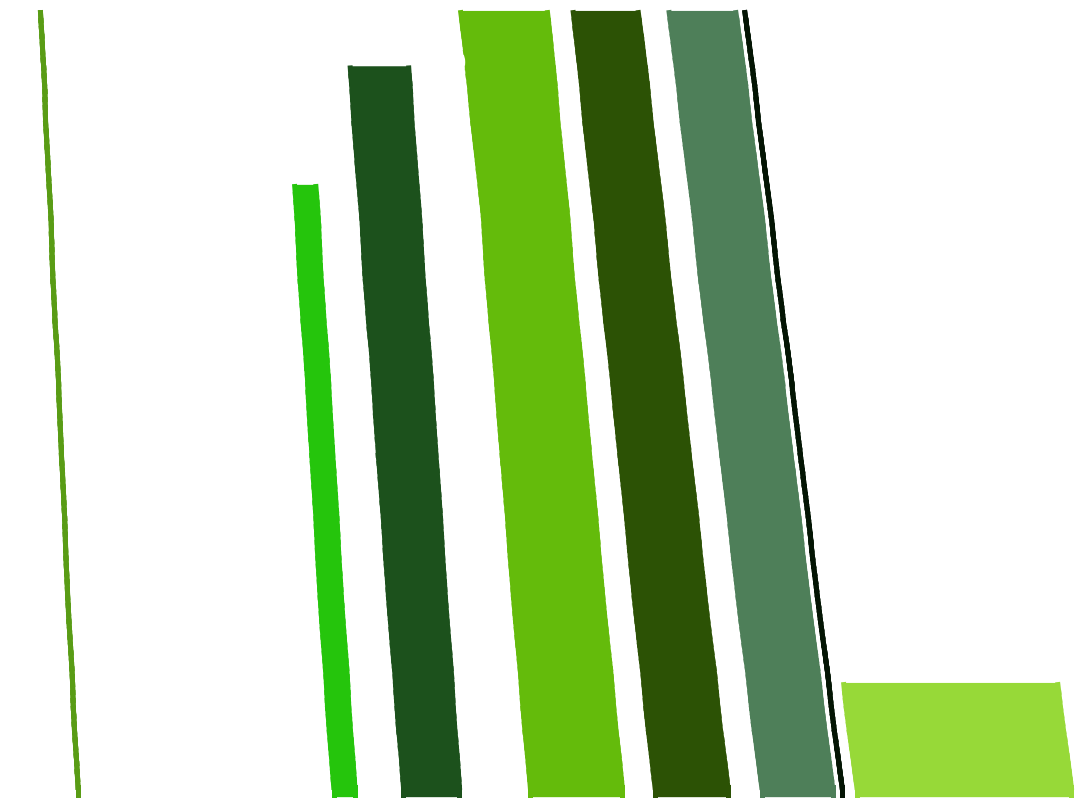
\includegraphics[width = 0.7 \textwidth]{./Diagrams/results/EPIs/292_8_102_7_34_8_dense.png}
\caption{Dense EPI corresponding to the strip on Figure~\ref{fig:strip4}}
\label{fig:dense4}
\end{figure}

\begin{figure}[h!]
\centering
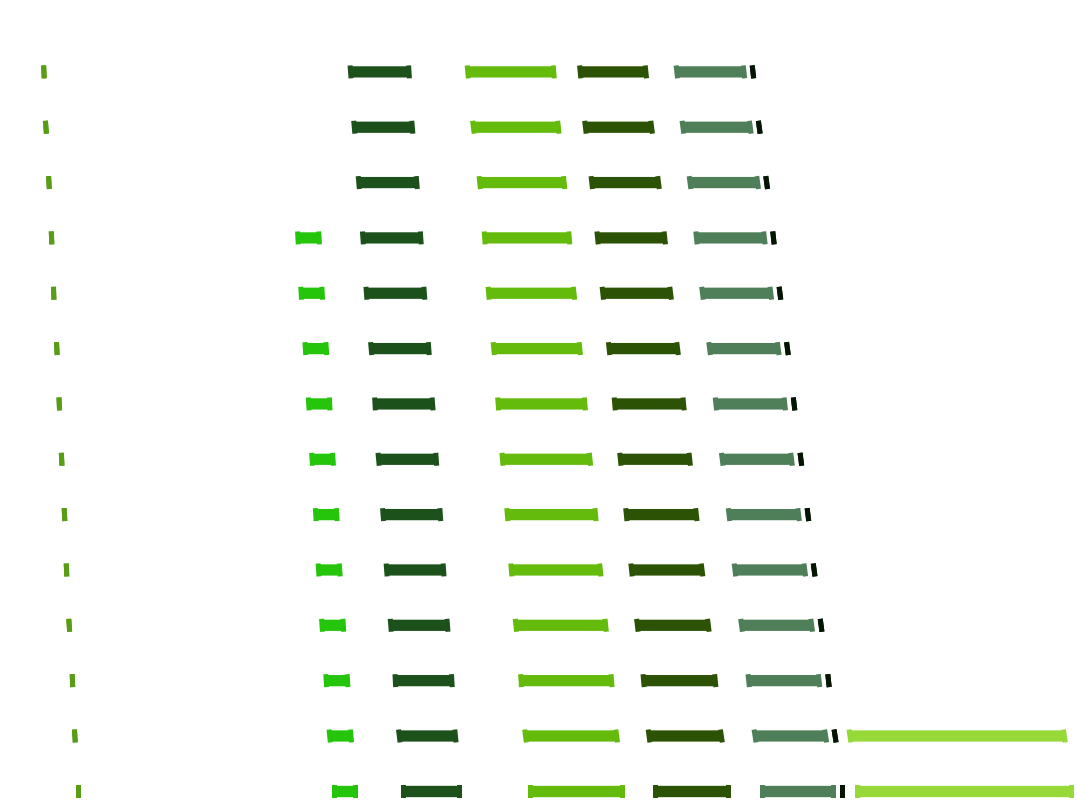
\includegraphics[width = 0.7 \textwidth]{./Diagrams/results/EPIs/292_8_102_7_34_8_sparse.png}
\caption{Sparse EPI corresponding to the strip on Figure~\ref{fig:strip4}}
\label{fig:sparse4}
\end{figure}

\begin{figure}[h!]
\centering
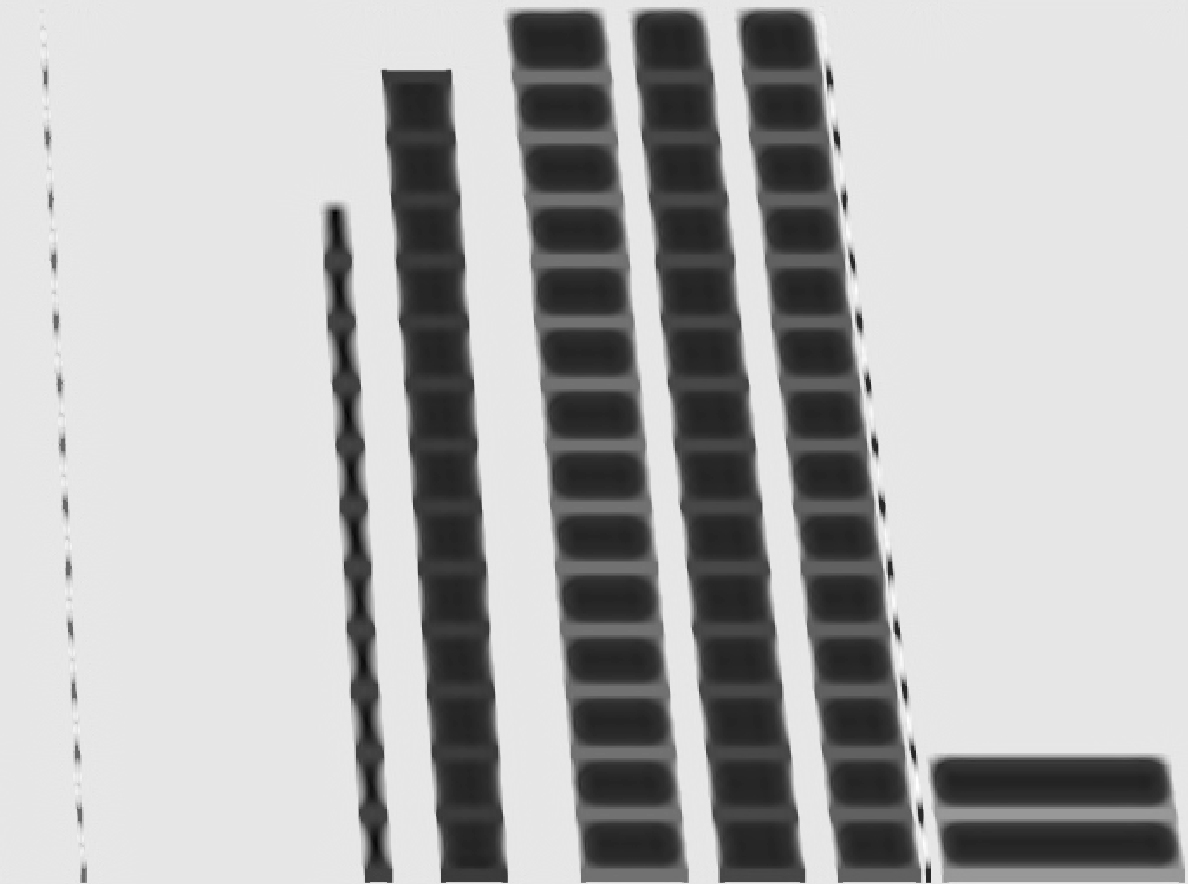
\includegraphics[width = 0.7 \textwidth]{./Diagrams/results/Inpainted/292_8_102_7_34_8_inpainted.png}
\caption{Inpainted EPI corresponding to the strip on Figure~\ref{fig:strip4}}
\label{fig:inpainted4}
\end{figure}


\begin{figure}[h!]
\centering
\includegraphics[width = 0.7 \textwidth]{./Diagrams/results/EPIs/673_10_102_4_48_8_strip.png}
\caption{Strip with tracked points}
\label{fig:strip5}
\end{figure}

\begin{figure}[h!]
\centering
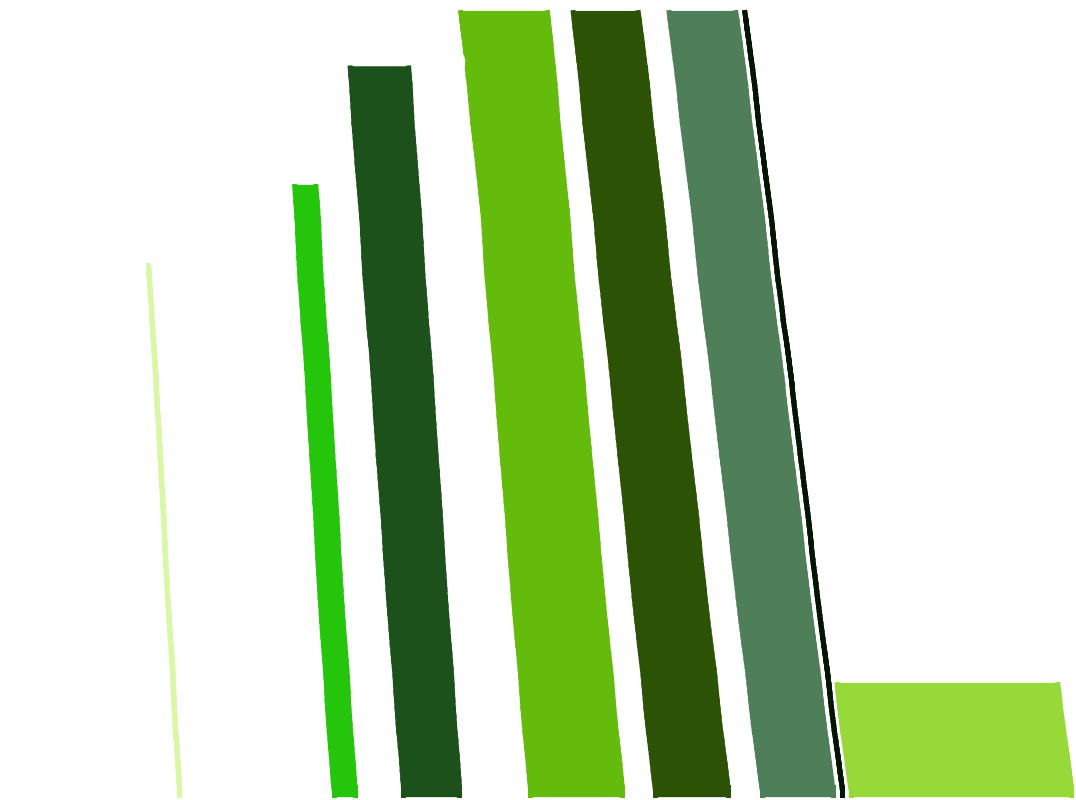
\includegraphics[width = 0.7 \textwidth]{./Diagrams/results/EPIs/673_10_102_7_48_8_dense.png}
\caption{Dense EPI corresponding to the strip on Figure~\ref{fig:strip5}}
\label{fig:dense5}
\end{figure}

\begin{figure}[h!]
\centering
\includegraphics[width = 0.7 \textwidth]{./Diagrams/results/EPIs/673_10_102_7_48_8_sparse.png}
\caption{Sparse EPI corresponding to the strip on Figure~\ref{fig:strip5}}
\label{fig:sparse5}
\end{figure}

\begin{figure}[h!]
\centering
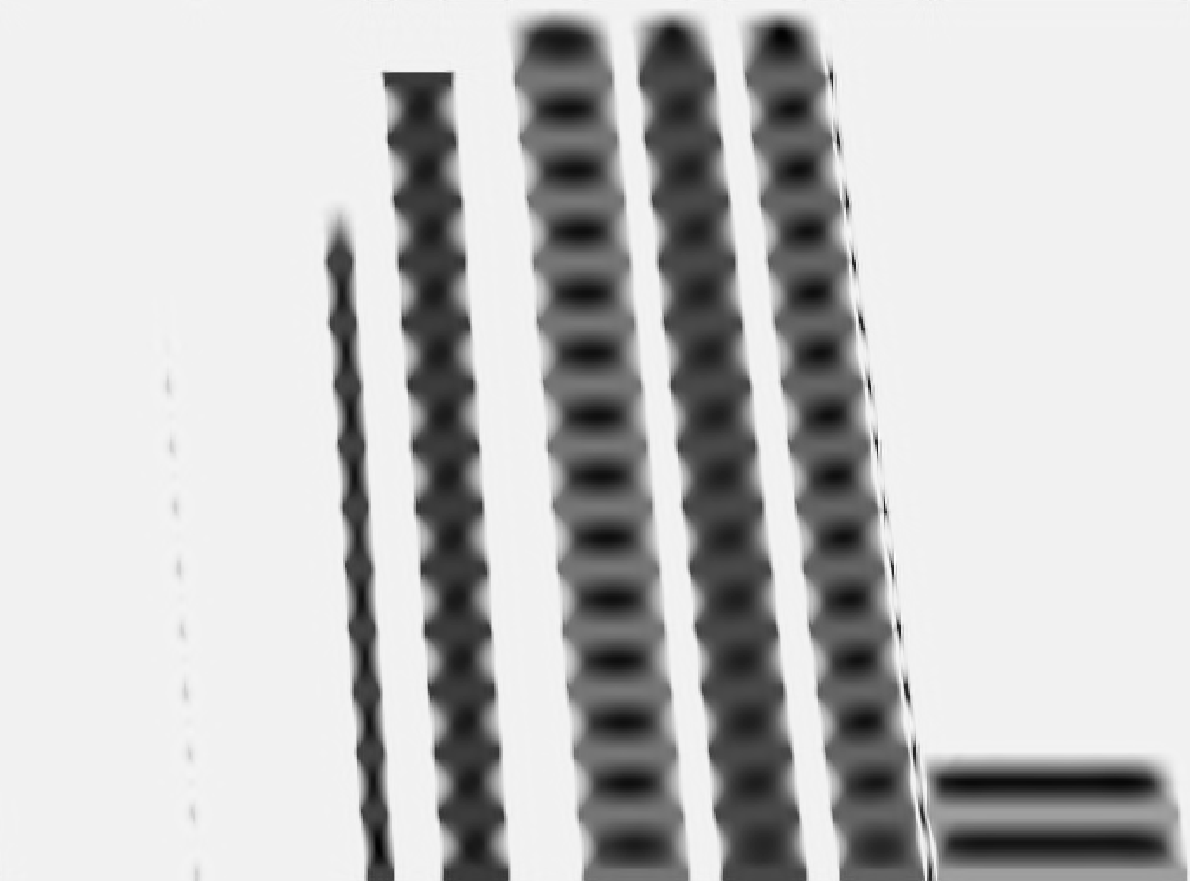
\includegraphics[width = 0.7 \textwidth]{./Diagrams/results/Inpainted/673_10_102_7_48_8_inpainted.png}
\caption{Inpainted EPI corresponding to the strip on Figure~\ref{fig:strip5}}
\label{fig:inpainted5}
\end{figure}

\item \textbf{Fourth step (line detection and depth map computation)}: We used Hough Line Transform on the inpainted EPIs to detect the lines and compute the depth map based on the slopes of the lines; this step will be explained in detail in the Section~\ref{sec:line_detect}.

\end{itemize}

\section{Line detection in inpainted EPIs and depth map computation}
\label{sec:line_detect}

Once we have the inpaited EPIs for our sparse set of views with disparity $d_{max}=7$ pixels, we need to be able to compute the slopes of the lines corresponding to different feature points, and then obtain the depth map; where the depth of a point corresponding to some line in an EPI will be given by Equation~\ref{eq:C1S4E2} in the form of

\begin{equation}
\label{eq:slope_epi}
D = h\frac{\Delta X}{\Delta U}= h\cdot \textrm{slope}
\end{equation}

where $h$ is the focal length of the camera that according to the specifications of the camera used in the data set is $h = 50mm=5\times 10^{-2}m$. In our case, each inpainted picture is imported in the line detection algorithm code as an image of certain $size=[size_x,size_y]$; by specifications of the data set we have that there were 101 taken pictures with a separation of $10$mm from each other with a total time span of $1100mm=1.1m$, the horizontal size in pixels of the used images in the data set is $683px$, therefore to obtain the depth of a point in Equation~\ref{eq:slope_epi} in an unified way and be able to compare the obtained depths in different strips we will need to modify the equation with a normalization term multiplying $m$, obtaining the equation:

\begin{equation}
\label{eq:slope_epi_unified}
D = (0.01m)\cdot \textrm{slope}\cdot\left(\frac{\textrm{size}_x}{\textrm{size}_y}\right)\cdot\left(\frac{1.1m}{683px}\right)
\end{equation}

\bigskip

The resulting depth given by Equation~\ref{eq:slope_epi_unified} has units of $\frac{m^2}{px}$, the transformation from pixels to meters is not straight forward since we would need to know the transformation betweeen the spatial and image coordinates, and for that one shouls know a priori the actual depth of some fixed point and the correspondance in meters of the pixels of features at that depth; therefore the obtained depth is relative, but that is enough to construct the depth map.

\bigskip

Now that we know how to get the depth of points by its slope in the corresponding epipolar plane image we need to have a way to actually measure slopes in lines on the inpainted epipolar planes images and therefore we need a method to detect lines in an image. There are different methods to detect lines in images, commonly known as edge detectors; one can give as examples the Canny edge detector, the Phase Stretch Transform (PST), the Sobel method and the Hough Line Transform (see \cite{LearnOpenCV}, \cite{MultipleView}, \cite{hough-duda}, \cite{hough-invented} for a detailed explanation of each of this methods). By its easy and fast implementation and its effectiveness we used the Hough line transform to detect lines on the inpainted EPIs. 

\bigskip

The Hough line transform was invented by Richard Duda and Peter Hart in 1972 on their paper "Use of the Hough Transformation to Detect Lines and Curves in Pictures"\cite{hough-duda} that is actually a generalization of a 1962 patent of Pual Hough\cite{hough-original} who proposed it for analysis of Bubble Chamber photographs for particle detection.

\bigskip

Even it seems as a trivial task for human vision, in automated analysis of digital images, a problem that often arises of detecting simple shapes as straight lines or circles. Generally an edge detector can be used as a pre-processing stage to obtain image points or image pixels that form part of the analysed curve in the image space. However imperfections in the image data or the edge detector may miss points or pixels on the desired cuves as well as spatial deviations between the ideal theoretical line/circle and the noisy edge points as they are obtained from the edge detector; therefore it is non-trivial to group the extracted edge features to an appropriate set of lines or circles. The Hough transform has a purpose address this problem by making it possible to perform groupings of edge points into object candidates by performing an explicit voting procedure over a set of parameterized image objects; in this thesis we will just make use of the simplest case of Hough transform that is detecting straight lines and it will be explained in the following.

\bigskip

A line in the image space can be expressed with two variables; for example by the parameters $(m,b)$ in Cartesian coordinates system where $m$ is the slope of the line and $b$ is the $y$-intercept of the line or in Polar coordinates system with parameters $(r,\theta)$ where $r$ is the distance to the origin and $\theta$ the angle with the $x$-axis. For Hough Transforms, we will express lines in the Polar system where a line equation can be written as:

\begin{equation}
\label{eq:polar-lines}
y = \left(-\frac{\cos\theta}{\sin\theta}\right)x+\left(\frac{r}{\sin\theta}\right)
\end{equation} 

this obtained by the relation $r=x\cos\theta+y\sin\theta$.

\bigskip

Given an arbitrary fixed point $(x_0,y_0)\in\mathbb{R}^2$, one can define a family of lines that goes through the poins by

\begin{equation}
\label{eq:family-lines}
r_{\theta}=x_0\cos\theta+y_0\sin\theta
\end{equation}

Therefore each pair $(r_{\theta},\theta)$ represents each line that passes by $(x_0,y_0)$.

\bigskip 

By the form of the Equation~\ref{eq:family-lines}, for a given fixed point $(x_0,y_0)$ the plot of the family of lines that goes through it $\theta\textrm{vs.}r_{\theta}$ is a sinusoid, we will consider only points such that $r>0$ and $0<\theta<2\pi$(see Figure~\ref{fig:family-lines-hough}).

\begin{figure}[h!]
\centering
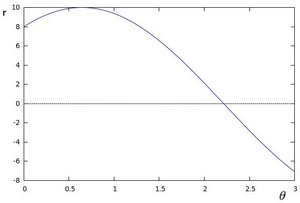
\includegraphics[width = 0.8 \textwidth]{./Diagrams/family-lines-hough.jpg}
\caption{Plot of $\theta\textrm{vs.}r_{\theta}$ for $x_0=8$ and $y_0=6$}
\label{fig:family-lines-hough}
\end{figure}

\bigskip

We can plot the sinusoidal curves of all the points in an image. If the curves of two different points intersect in the plane $\theta-r_{\theta}$, it means that both points belong to a same line; see the example in Figure~\ref{fig:intersection-hough}.

\begin{figure}[h!]
\centering
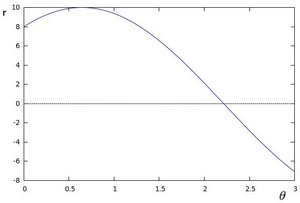
\includegraphics[width = 0.8 \textwidth]{./Diagrams/family-lines-hough.jpg}
\caption{Plot of $\theta\textrm{vs.}r_{\theta}$ corresponding to the points $(x_0,y_0)=(8,6)$, $(x_1,y_1)=(4,9)$ and $(x_2,y_2)=(12,3)$}
\label{fig:intersection-hough}
\end{figure}

\bigskip

The three plots in Figure~\ref{fig:intersection-hough} intersect in one single point $(0.925,9.6)$, these coordinates are the parameters $(\theta,r)$ or the line in which $(x_0,y_0)$, $(x_1,y_1)$ and $(x_2,y_2)$ lay; therefore in general, a line can be \textbf{detected} by finding the number of intersections between curves. The more curves intersecting means that the line represented by that intersection have more points. In general we can define a threshold of the minimum number of intersections needed to detect a line. This is what the Hough Line Transform does. It keeps track of the intersection between curves of every point in the image. If the number of intersections is above some threshold, then it declares it as a line with the parameters $(\theta,r_{\theta})$ of the intersection point.

\bigskip 

There are different existing implementations of the Hough line, in Python, C++ and Matlab; in this thesis we used the python implementation using the OpenCV API in python, cause is very simple to use and fast to run; we make use of the Canny edge detector that is similar to the already explained Shi-Tomasi and for more detail one should check \cite{LearnOpenCV} and the Hough Line Transfom. In order to compute the depth map, we make use of the inpainted EPIs corresponding to strips at different fixed $y$'s; the points were divided by the different features were they belong, those features are enumerated in the following list and pictured in Figure~\ref{feature_points.png}

\begin{enumerate}
\item Bush 1.
\item Bush 2.
\item Bush 3. 
\item Tree 1.
\item Tree 2.
\item Tree 3.
\item Tree 4.
\item Tree 5.
\item Tree 6.
\item Lamp Post 1.
\item Lamp Post 2.
\item Front Wall.
\item Window 1.
\item Window 2. 
\item Window 3. 
\item Window 4.
\item Pillar 1.  
\item Pillar 2. 
\item Cable 1.
\item Cable 2.
\item Cable 3.
\item High Lamp.
\item Tower.
\end{enumerate} 

\begin{figure}[h!]
\centering
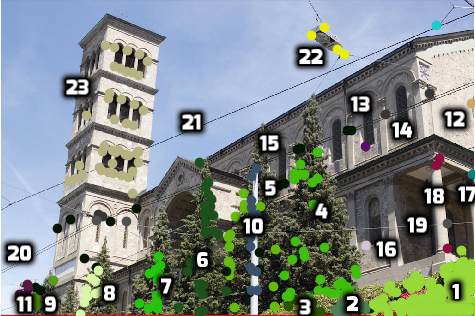
\includegraphics[width = 0.9 \textwidth]{./Diagrams/results/data_set/feature_points.png}
\caption{Features of the Church with tracked points}
\label{fig:feature_points}
\end{figure}

Once we have points associated to features, we compute the depth of this points at different fixed $y$-strips finding out that for a fixed $y$-strip the points of a certain feature have relatively the same depth, therefore we assigned a depth to a feature for a fixed $y$. As we already mentioned we used the OpenCV python API as well as some python code for computing the depth map with this method, the code can be found in Appendix~\ref{sec:Appendix_D} and the obtained results are in the tables~\ref{table1} to~\ref{table6} where the values at each height $y$ (where the different strips are centered at) are the obtained depth of the points of that feature at that height in meters$^2$/pixels and whenever occur a blank space means that such feature has not points in such height (is worth to mention that the heights are measured from bottom to top, i.e.\ the bigger the height, the lower in the picture); this values describe completly the depth map, if one would like to visualize them in a refocusing-type application we should perform the so called light field rendering, where one finds contours of the corresponding features and apply a gaussian filter to defocused the elements that are not at the same depth, but this is not part of this thesis and will be taken as a future development goal. One can use as a guide of the heights Figure~\ref{feature_points_grid}. 

\begin{figure}[h!]
\centering
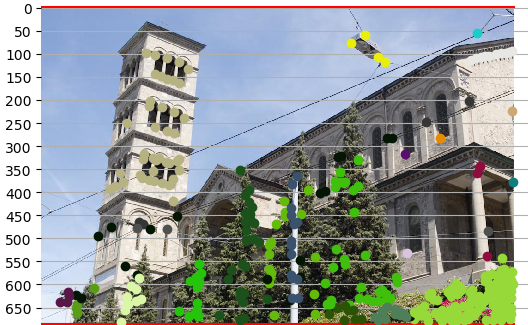
\includegraphics[width = 0.9 \textwidth]{./Diagrams/results/data_set/feature_points_grid.png}
\caption{Features of the Church with tracked points with grid of heights}
\label{fig:feature_points_grid}
\end{figure}


\begin{table}[!htb]
\centering
    \begin{tabular}{| c | c | c | c | c | c | c | c | c |}
    \hline
    feature/height(px) & 680 & 673 & 664 & 632 & 616 & 600 & 584 & 568 \\ \hline
		 Bush1 & 0.0161 & 0.0157 & 0.0158 & 0.0156 & 0.0157 & 0.0161 & 0.0160 & 0.0158\\ \hline
		 Bush2 & 0.0217 & 0.0221 & 0.0221 & 0.0220 &  &  &  & \\ \hline	
		 Bush3 & 0.0257 & 0.0261 & 0.0260 & 0.0258 & 0.0258 &  &  & \\ \hline	
		 Tree1 & 0.0284 & 0.0285 & 0.0286 & 0.0285 & 0.0285 & 0.0286 & 0.0287 & 0.0291 \\ \hline	
		 Tree2 &  &  & 0.0442  &  &  & 0.045  & 0.046 & 0.045 \\ \hline	
		 Tree3 & 0.0501 & 0.0502 & 0.0501 & 0.0499 & 0.0498 & 0.0502 & 0.0500 & 0.0501\\ \hline	
		 Tree4 & 0.0594 & 0.0591 & 0.0590 & 0.0589 & 0.0590 & 0.0593 & 0.0595 & 0.0594\\ \hline	
		 Tree5 & 0.0801 & 0.0799 & 0.0798 & 0.0800 & 0.0801 & 0.0798 & 0.0799 & 0.0800\\ \hline	
		 Tree6 & 0.1001 & 0.0998 & 0.0999 & 0.0998 & 0.1003 & 0.1002 &  & \\ \hline	
     LampPost1 &  &  & & 0.0181 &  & 0.0180 & 0.0182 &  \\ \hline
		 LampPost2 &  &  &  & 0.1123 & 0.1122  &  &  & \\ \hline
		 FrontWall &  &  &  &  &  &  &  & \\ \hline
		 Window1 &  &  &  &  &  &  &  & \\ \hline
		 Window2 &  &  &  &  &  &  &  & \\ \hline
		 Window3 &  &  &  &  &  &  &  & \\ \hline
		 Window4 &  &  &  &  &  &  &  & \\ \hline
		 Pillar1 &  &  &  &  &  &  &  & \\ \hline
		 Pillar2 &  &  &  &  &  &  &  & \\ \hline
		 Cable1 &  &  &  &  &  &  &  & \\ \hline
	   Cable2 &  &  &  &  &  &  &  & \\ \hline
	   Cable3 &  &  &  &  &  &  &  & \\ \hline
		 HighLamp &  &  &  &  &  &  &  & \\ \hline
	   Tower &  &  &  &  &  &  &  & \\ \hline
    \end{tabular}
		\caption{Depth of features in $m^2/px$ at different heights in $px$}\label{table1}
\end{table}

\begin{table}[!htb]
\centering
    \begin{tabular}{| c | c | c | c | c | c | c | c | c |}
    \hline
    feature/height(px) & 552 & 536 & 520 & 504 & 488 & 472 & 456 & 440\\ \hline
		 Bush1 & 0.0157 &  &  &  &  &  &  & \\ \hline
		 Bush2 &  &  &  &  &  &  &  & \\ \hline	
		 Bush3 &  &  &  &  &  &  &  & \\ \hline	
		 Tree1 & 0.0291 & 0.0292 & 0.0290 & 0.0291 &  &  &  & 0.030 \\ \hline	
		 Tree2 & 0.0461 & 0.0456 & 0.0460 & 0.0459 &  &  & 0.0461 & 0.0461\\ \hline	
		 Tree3 & 0.0495 & 0.0496 &  & 0.0497 & 0.0498 & 0.0499 & 0.0495 & 0.0501 \\ \hline	
		 Tree4 & 0.0594 &  &  &  &  &  &  & \\ \hline	
		 Tree5 &  &  &  &  &  &  &  & \\ \hline	
		 Tree6 &  &  &  &  &  &  &  & \\ \hline	
     LampPost1 & 0.0181 & 0.0180 & 0.0182 & 0.0183 &  & 0.0182 & 0.0179 & 0.0180 \\ \hline
		 LampPost2 &  &  &  &  &  &  &  & \\ \hline
		 FrontWall &  &  &  &  &  &  &  & \\ \hline
		 Window1 &  &  &  &  &  &  &  & \\ \hline
		 Window2 &  &  &  &  &  &  &  & \\ \hline
		 Window3 &  &  &  &  &  &  &  & \\ \hline
		 Window4 &  & 0.0391 &  &  &  &  &  & \\ \hline
		 Pillar1 &  &  &  &  &  &  &  & 0.0054 \\ \hline
		 Pillar2 &  & 0.0251 &  &  &  &  &  & \\ \hline
		 Cable1 &  &  &  &  & 0.0020 &  &  & \\ \hline
	   Cable2 &  &  &  &  &  & 0.0701 & 0.0608 & \\ \hline
	   Cable3 &  &  &  &  &  &  &  & \\ \hline
		 HighLamp &  &  &  &  &  &  &  & \\ \hline
	   Tower &  &  &  &  &  &  &  & \\ \hline
    \end{tabular}
		\caption{Depth of features in $m^2/px$ at different heights in $px$}\label{table2}
\end{table}

\begin{table}[!htb]
\centering
    \begin{tabular}{| c | c | c | c | c | c | c | c | c |}
    \hline
    feature/height(px) & 424 & 408 & 392 & 376 & 360 & 344 & 328 & 322\\ \hline
		 Bush1 &   &   &  &  &  &  &  & \\ \hline
		 Bush2 &  &  &  &  &  &  &  & \\ \hline	
		 Bush3 &  &  &  &  &  &  &  & \\ \hline	
		 Tree1 &  &  & 0.0332 & 0.0341 & 0.0341 &  & 0.0335 & \\ \hline	
		 Tree2 &  & 0.0459 &  &  &  &  &  & \\ \hline	
		 Tree3 & 0.0502 & 0.0500 & 0.0501 &  & 0.0502 & 0.0499 &  & \\ \hline	
		 Tree4 &  &  &  &  &  &  &  & \\ \hline	
		 Tree5 &  &  &  &  &  &  &  & \\ \hline	
		 Tree6 &  &  &  &  &  &  &  & \\ \hline	
     LampPost1 &  &  &  &  & 0.0180 & 0.0181 &  & \\ \hline
		 LampPost2 &  &  &  &  &  &  &  & \\ \hline
		 FrontWall &  &  &  &  &  &  &  & \\ \hline
		 Window1 &  &  &  &  &  &  &  & 0.0601\\ \hline
		 Window2 &  &  &  &  &  &  &  & \\ \hline
		 Window3 &  & 0.0522 &  &  &  &  &  & \\ \hline
		 Window4 &  &  &  &  &  &  &  & \\ \hline
		 Pillar1 &  &  &  &  &  &  &  & \\ \hline
		 Pillar2 &  &  &  &  &  & 0.0256 &  & \\ \hline
		 Cable1 &  &  &  &  &  &  & & \\ \hline
	   Cable2 &  &  &  &  &  &  & 0.0212 & \\ \hline
	   Cable3 &  &  &  &  &  &  &  & \\ \hline
		 HighLamp &  &  &  &  &  &  &  & \\ \hline
	   Tower & 0.0995 &  & 0.1002  & 0.1003  & 0.1002 & 0.1001 & 0.1002 & 0.0996 \\ \hline
    \end{tabular}
		\caption{Depth of features in $m^2/px$ at different heights in $px$}\label{table3}
\end{table}

\begin{table}[!htb]
\centering
    \begin{tabular}{| c | c | c | c | c | c | c | c | c |}
    \hline
    feature/height(px) & 312 & 306 & 300 & 292 & 280 & 264 & 248 & 232 \\ \hline
		 Bush1 &  &  &  &  &  &  &  & \\ \hline
		 Bush2 &  &  &  &  &  &  &  & \\ \hline	
		 Bush3 &  &  &  &  &  &  &  & \\ \hline	
		 Tree1 &  &  &  &  &  &  &  & \\ \hline	
		 Tree2 &  &  &  &  &  &  &  & \\ \hline	
		 Tree3 &  &  &  &  &  &  &  & \\ \hline	
		 Tree4 &  &  &  &  &  &  &  & \\ \hline	
		 Tree5 &  &  &  &  &  &  &  & \\ \hline	
		 Tree6 &  &  &  &  &  &  &  & \\ \hline	
     LampPost1 &  &  &  &  &  &  &  & \\ \hline
		 LampPost2 &  &  &  &  &  &  &  & \\ \hline
		 FrontWall &  &  &  &  &  &  &  & 0.0051\\ \hline
		 Window1 &  &  &  &  &  &  &  & \\ \hline
		 Window2 &  &  &  &  & 0.0402 &  &  & \\ \hline
		 Window3 &  &  &  &  &  &  &  & \\ \hline
		 Window4 &  &  &  &  &  &  &  & \\ \hline
		 Pillar1 &  &  &  &  &  &  &  & \\ \hline
		 Pillar2 &  &  &  &  &  &  &  & \\ \hline
		 Cable1 &  &  &  &  &  &  &  & \\ \hline
	   Cable2 &  &  &  &  & 0.0131 &  &  & \\ \hline
	   Cable3 &  &  &  &  &  &  &  & \\ \hline
		 HighLamp &  &  &  &  &  &  &  & \\ \hline
	   Tower &  &  &  &  &  & 0.1001 & 0.0999 & 0.1003 \\ \hline
    \end{tabular}
		\caption{Depth of features in $m^2/px$ at different heights in $px$}\label{table4}
\end{table}

\begin{table}[!htb]
\centering
    \begin{tabular}{| c | c | c | c | c | c | c | c | c |}
    \hline
    feature/height(px) & 216 & 200 & 168 & 152 & 136 & 120 & 104 & 88\\ \hline
		 Bush1 &  &  &  &  &  &  &  & \\ \hline
		 Bush2 &  &  &  &  &  &  &  & \\ \hline	
		 Bush3 &  &  &  &  &  &  &  & \\ \hline	
		 Tree1 &  &  &  &  &  &  &  & \\ \hline	
		 Tree2 &  &  &  &  &  &  &  & \\ \hline	
		 Tree3 &  &  &  &  &  &  &  & \\ \hline	
		 Tree4 &  &  &  &  &  &  &  & \\ \hline	
		 Tree5 &  &  &  &  &  &  &  & \\ \hline	
		 Tree6 &  &  &  &  &  &  &  & \\ \hline	
     LampPost1 &  &  &  &  &  &  &  & \\ \hline
		 LampPost2 &  &  &  &  &  &  &  & \\ \hline
		 FrontWall &  &  &  &  &  &  &  & \\ \hline
		 Window1 &  &  &  &  &  &  &  & \\ \hline
		 Window2 &  &  &  &  &  &  &  & \\ \hline
		 Window3 &  &  &  &  &  &  &  & \\ \hline
		 Window4 &  &  &  &  &  &  &  & \\ \hline
		 Pillar1 &  &  &  &  &  &  &  & \\ \hline
		 Pillar2 &  &  &  &  &  &  &  & \\ \hline
		 Cable1 &  &  &  &  &  &  &  & \\ \hline
	   Cable2 &  & 0.0015 &  &  &  &  &  & \\ \hline
	   Cable3 &  &  &  &  &  &  &  & \\ \hline
		 HighLamp &  &  &  &  &  & 0.0009 &  & \\ \hline
	   Tower & 0.1002 & 0.0998 &  & 0.0999 & 0.1002 & 0.0998 & 0.1001 & \\ \hline
    \end{tabular}
		\caption{Depth of features in $m^2/px$ at different heights in $px$}\label{table5}
\end{table}

\begin{table}[!htb]
\centering
    \begin{tabular}{| c | c | c | c | c | c | c | c | c |}
    \hline
    feature/height(px) & 72 & 56\\ \hline
		 Bush1 &  &  \\ \hline
		 Bush2 &  &  \\ \hline	
		 Bush3 &  &  \\ \hline	
		 Tree1 &  &  \\ \hline	
		 Tree2 &  &   \\ \hline	
		 Tree3 &  &   \\ \hline	
		 Tree4 &  &   \\ \hline	
		 Tree5 &  &   \\ \hline	
		 Tree6 &  &    \\ \hline	
     LampPost1 &  &  \\ \hline
		 LampPost2 &  &  \\ \hline
		 FrontWall &  &  \\ \hline
		 Window1 &  &  \\ \hline
		 Window2 &  &  \\ \hline
		 Window3 &  &  \\ \hline
		 Window4 &  &  \\ \hline
		 Pillar1 &  &   \\ \hline
		 Pillar2 &  &  \\ \hline
		 Cable1 &  &  \\ \hline
	   Cable2 &  &  \\ \hline
	   Cable3 &  & 0.0020\\ \hline
		 HighLamp & 0.0008 & 0.0007  \\ \hline
	   Tower &  & \\ \hline
    \end{tabular}
		\caption{Depth of features in $m^2/px$ at different heights in $px$}\label{table6}
\end{table}

It could also be interesting to have depth map not by feature but by $x$ position, therefore one could make a heat map with the depth which will give us a more effective way to analyse it; the issue with this approach is that hardly more than the already tracked points can be tracked by the common tracking algorithms; this could be improved in the future using some other transformation like iterative feature extractors like Convolutional Neural Networks\cite{DCNN} to have a better corner detector and to be able to track more points; even though this approach works very well and the comparison with the existent light field recovery methods for approaching the depth map of a scene, in the next section we will shortly review this. 

\section{Performance and results comparison with previews works}

We already mentioned several times the computer system that was used is a low end MacBook whose processor and gpu are by far not the best in the commercial market and are even worse in comparison with the high-end servers used some researcher on the area. 

\bigskip

In the last sections we got the next running times on finishing the whole pipeline of light field reconstruction:

\begin{itemize}
\item \textbf{Point tracking}: 16.36 seconds.
\item \textbf{Sparse EPI painting}: 9.46 seconds (43 EPIs, 0.22 seconds for each).
\item \textbf{Sparse EPI inpainting}: 666.50 (43 inpeinted EPIs, 15.50 seconds for each).
\item \textbf{Line detection and depth map computation}: 0.43 seconds (43 EPIs, 0.01 seconds for each).
\end{itemize}

This gives a total of 692.75 seconds to reconstruct the Light Field and compute the Depth Map. 
